% Options for packages loaded elsewhere
\PassOptionsToPackage{unicode}{hyperref}
\PassOptionsToPackage{hyphens}{url}
\PassOptionsToPackage{dvipsnames,svgnames,x11names}{xcolor}
%
\documentclass[
  letterpaper,
  DIV=11,
  numbers=noendperiod]{scrreprt}

\usepackage{amsmath,amssymb}
\usepackage{iftex}
\ifPDFTeX
  \usepackage[T1]{fontenc}
  \usepackage[utf8]{inputenc}
  \usepackage{textcomp} % provide euro and other symbols
\else % if luatex or xetex
  \usepackage{unicode-math}
  \defaultfontfeatures{Scale=MatchLowercase}
  \defaultfontfeatures[\rmfamily]{Ligatures=TeX,Scale=1}
\fi
\usepackage{lmodern}
\ifPDFTeX\else  
    % xetex/luatex font selection
\fi
% Use upquote if available, for straight quotes in verbatim environments
\IfFileExists{upquote.sty}{\usepackage{upquote}}{}
\IfFileExists{microtype.sty}{% use microtype if available
  \usepackage[]{microtype}
  \UseMicrotypeSet[protrusion]{basicmath} % disable protrusion for tt fonts
}{}
\makeatletter
\@ifundefined{KOMAClassName}{% if non-KOMA class
  \IfFileExists{parskip.sty}{%
    \usepackage{parskip}
  }{% else
    \setlength{\parindent}{0pt}
    \setlength{\parskip}{6pt plus 2pt minus 1pt}}
}{% if KOMA class
  \KOMAoptions{parskip=half}}
\makeatother
\usepackage{xcolor}
\setlength{\emergencystretch}{3em} % prevent overfull lines
\setcounter{secnumdepth}{5}
% Make \paragraph and \subparagraph free-standing
\ifx\paragraph\undefined\else
  \let\oldparagraph\paragraph
  \renewcommand{\paragraph}[1]{\oldparagraph{#1}\mbox{}}
\fi
\ifx\subparagraph\undefined\else
  \let\oldsubparagraph\subparagraph
  \renewcommand{\subparagraph}[1]{\oldsubparagraph{#1}\mbox{}}
\fi


\providecommand{\tightlist}{%
  \setlength{\itemsep}{0pt}\setlength{\parskip}{0pt}}\usepackage{longtable,booktabs,array}
\usepackage{calc} % for calculating minipage widths
% Correct order of tables after \paragraph or \subparagraph
\usepackage{etoolbox}
\makeatletter
\patchcmd\longtable{\par}{\if@noskipsec\mbox{}\fi\par}{}{}
\makeatother
% Allow footnotes in longtable head/foot
\IfFileExists{footnotehyper.sty}{\usepackage{footnotehyper}}{\usepackage{footnote}}
\makesavenoteenv{longtable}
\usepackage{graphicx}
\makeatletter
\def\maxwidth{\ifdim\Gin@nat@width>\linewidth\linewidth\else\Gin@nat@width\fi}
\def\maxheight{\ifdim\Gin@nat@height>\textheight\textheight\else\Gin@nat@height\fi}
\makeatother
% Scale images if necessary, so that they will not overflow the page
% margins by default, and it is still possible to overwrite the defaults
% using explicit options in \includegraphics[width, height, ...]{}
\setkeys{Gin}{width=\maxwidth,height=\maxheight,keepaspectratio}
% Set default figure placement to htbp
\makeatletter
\def\fps@figure{htbp}
\makeatother
\newlength{\cslhangindent}
\setlength{\cslhangindent}{1.5em}
\newlength{\csllabelwidth}
\setlength{\csllabelwidth}{3em}
\newlength{\cslentryspacingunit} % times entry-spacing
\setlength{\cslentryspacingunit}{\parskip}
\newenvironment{CSLReferences}[2] % #1 hanging-ident, #2 entry spacing
 {% don't indent paragraphs
  \setlength{\parindent}{0pt}
  % turn on hanging indent if param 1 is 1
  \ifodd #1
  \let\oldpar\par
  \def\par{\hangindent=\cslhangindent\oldpar}
  \fi
  % set entry spacing
  \setlength{\parskip}{#2\cslentryspacingunit}
 }%
 {}
\usepackage{calc}
\newcommand{\CSLBlock}[1]{#1\hfill\break}
\newcommand{\CSLLeftMargin}[1]{\parbox[t]{\csllabelwidth}{#1}}
\newcommand{\CSLRightInline}[1]{\parbox[t]{\linewidth - \csllabelwidth}{#1}\break}
\newcommand{\CSLIndent}[1]{\hspace{\cslhangindent}#1}

\KOMAoption{captions}{tableheading}
\makeatletter
\@ifpackageloaded{tcolorbox}{}{\usepackage[skins,breakable]{tcolorbox}}
\@ifpackageloaded{fontawesome5}{}{\usepackage{fontawesome5}}
\definecolor{quarto-callout-color}{HTML}{909090}
\definecolor{quarto-callout-note-color}{HTML}{0758E5}
\definecolor{quarto-callout-important-color}{HTML}{CC1914}
\definecolor{quarto-callout-warning-color}{HTML}{EB9113}
\definecolor{quarto-callout-tip-color}{HTML}{00A047}
\definecolor{quarto-callout-caution-color}{HTML}{FC5300}
\definecolor{quarto-callout-color-frame}{HTML}{acacac}
\definecolor{quarto-callout-note-color-frame}{HTML}{4582ec}
\definecolor{quarto-callout-important-color-frame}{HTML}{d9534f}
\definecolor{quarto-callout-warning-color-frame}{HTML}{f0ad4e}
\definecolor{quarto-callout-tip-color-frame}{HTML}{02b875}
\definecolor{quarto-callout-caution-color-frame}{HTML}{fd7e14}
\makeatother
\makeatletter
\makeatother
\makeatletter
\@ifpackageloaded{bookmark}{}{\usepackage{bookmark}}
\makeatother
\makeatletter
\@ifpackageloaded{caption}{}{\usepackage{caption}}
\AtBeginDocument{%
\ifdefined\contentsname
  \renewcommand*\contentsname{Table of contents}
\else
  \newcommand\contentsname{Table of contents}
\fi
\ifdefined\listfigurename
  \renewcommand*\listfigurename{List of Figures}
\else
  \newcommand\listfigurename{List of Figures}
\fi
\ifdefined\listtablename
  \renewcommand*\listtablename{List of Tables}
\else
  \newcommand\listtablename{List of Tables}
\fi
\ifdefined\figurename
  \renewcommand*\figurename{Figure}
\else
  \newcommand\figurename{Figure}
\fi
\ifdefined\tablename
  \renewcommand*\tablename{Table}
\else
  \newcommand\tablename{Table}
\fi
}
\@ifpackageloaded{float}{}{\usepackage{float}}
\floatstyle{ruled}
\@ifundefined{c@chapter}{\newfloat{codelisting}{h}{lop}}{\newfloat{codelisting}{h}{lop}[chapter]}
\floatname{codelisting}{Listing}
\newcommand*\listoflistings{\listof{codelisting}{List of Listings}}
\makeatother
\makeatletter
\@ifpackageloaded{caption}{}{\usepackage{caption}}
\@ifpackageloaded{subcaption}{}{\usepackage{subcaption}}
\makeatother
\makeatletter
\@ifpackageloaded{tcolorbox}{}{\usepackage[skins,breakable]{tcolorbox}}
\makeatother
\makeatletter
\@ifundefined{shadecolor}{\definecolor{shadecolor}{rgb}{.97, .97, .97}}
\makeatother
\makeatletter
\makeatother
\makeatletter
\makeatother
\ifLuaTeX
  \usepackage{selnolig}  % disable illegal ligatures
\fi
\IfFileExists{bookmark.sty}{\usepackage{bookmark}}{\usepackage{hyperref}}
\IfFileExists{xurl.sty}{\usepackage{xurl}}{} % add URL line breaks if available
\urlstyle{same} % disable monospaced font for URLs
\hypersetup{
  pdftitle={MA32009},
  pdfauthor={Philip Murray},
  colorlinks=true,
  linkcolor={blue},
  filecolor={Maroon},
  citecolor={Blue},
  urlcolor={Blue},
  pdfcreator={LaTeX via pandoc}}

\title{MA32009}
\author{Philip Murray}
\date{2023-12-22}

\begin{document}
\maketitle
\ifdefined\Shaded\renewenvironment{Shaded}{\begin{tcolorbox}[breakable, sharp corners, borderline west={3pt}{0pt}{shadecolor}, interior hidden, boxrule=0pt, frame hidden, enhanced]}{\end{tcolorbox}}\fi

\renewcommand*\contentsname{Table of contents}
{
\hypersetup{linkcolor=}
\setcounter{tocdepth}{2}
\tableofcontents
}
\bookmarksetup{startatroot}

\hypertarget{preface}{%
\chapter*{Preface}\label{preface}}
\addcontentsline{toc}{chapter}{Preface}

\markboth{Preface}{Preface}

Welcome to MA42002 Mathematical Biology I.

My name is Philip Murray and I am the module lead.

\hypertarget{how-to-contact-me}{%
\section*{How to contact me?}\label{how-to-contact-me}}
\addcontentsline{toc}{section}{How to contact me?}

\markright{How to contact me?}

\begin{itemize}
\tightlist
\item
  email: pmurray@dundee.ac.uk
\item
  office: G11, Fulton Building
\end{itemize}

\hypertarget{lecture-notes}{%
\section*{Lecture notes}\label{lecture-notes}}
\addcontentsline{toc}{section}{Lecture notes}

\markright{Lecture notes}

You can find lecture notes for the module on this page. If you would
like a pdf this can be easily generated by clicking on the pdf link on
the top left of the webpages. I will occasionally edit/update the notes
we proceed through lectures. If you spot any errors, typos or omissions
please let me know.

\hypertarget{reading}{%
\section*{Reading}\label{reading}}
\addcontentsline{toc}{section}{Reading}

\markright{Reading}

Mathematical Biology I, Murray (2002)

Esswential Mathemtical Biology Britton and Britton (2003)

Mathematical models in Biology Edelstein-Keshet (2005)

\hypertarget{python-codes}{%
\section*{Python codes}\label{python-codes}}
\addcontentsline{toc}{section}{Python codes}

\markright{Python codes}

I have provided Python codes for most of the figures in the notes (you
can unfold code section by clicking `Code'). Note that the Python code
does not appear in the pdf.

Many of you have taken the Introduction to Programming module at Level 2
and have therefore some experience using Python. I strongly encourage
you to use the provided codes as a tool to play around with numerical
solutions of the various models that we will be working on. The codes
should run as standalone Python codes.

\hypertarget{references}{%
\section*{References}\label{references}}
\addcontentsline{toc}{section}{References}

\markright{References}

\part{Discrete time}

\hypertarget{single-species-population-dynamics}{%
\chapter{Single species population
dynamics}\label{single-species-population-dynamics}}

Let us firstly consider models of a single population defined at
discrete times. Discrete (rather than continuous) time is used in
population models where, for example, there are strong annual trends in
the underlying animal behaviour (e.g.~fish eggs hatching at a fixed time
in the year), there are not overlapping generations and the population
size at the next time step can be written as a function of the current
population size.

\hypertarget{a-general-model-for-a-single-population-in-discrete-time}{%
\section{A general model for a single population in discrete
time}\label{a-general-model-for-a-single-population-in-discrete-time}}

Let \(t\) be an independent variable representing time and \(N_t\) be a
dependent variable representing the size of the population of a given
species at time \(t\).

Consider the first order difference equation
\begin{equation}\protect\hypertarget{eq-GeneralPopulationModel}{}{
N_{t+1}=N_tf(N_t)=H(N_t),
}\label{eq-GeneralPopulationModel}\end{equation} where \(f(N_t)\) is a
function that defines the per capita growth rate. The function
\(H(N_t)\) describes the total (net) growth rate.

Given some initial condition \(N_0\) defined such that \[
N_{t=0}=N_0,
\] the goal of this section is to develop a range of techniques that
allow us to analyse the behaviour of
Equation~\ref{eq-GeneralPopulationModel} for a given \(H\).

Finally, note that many of you were introduced to difference equations
in the module MA21003 Discrete Mathematics. It is recommended that you
revisit the section on Discrete Difference Equations.

\hypertarget{the-malthusian-model}{%
\section{The Malthusian model}\label{the-malthusian-model}}

Perhaps the simplest form for equation
Equation~\ref{eq-GeneralPopulationModel} is when the net per capita
growth rate is a constant.

Let \(b\) be the per capita growth rate and \(d\) the per capita death
rate with \(b\) and \(d\) both positive real constants.

Hence, a population of size \(N_t\) at time \(t\) will grow by \[
bN_t
\] over the course of the next iteration and decay by\\
\[
dN_t.
\] Therefore the population size at time \(t+1\) is
\begin{equation}\protect\hypertarget{eq-MalthusianEqn}{}{
N_{t+1}=N_t + bN_t - dN_t=rN_t,
}\label{eq-MalthusianEqn}\end{equation} where the parameter \(r=1+b-d\)
is known as the net growth rate.

Given the initial condition \(N_0\), equation
Equation~\ref{eq-MalthusianEqn} can be solved recursively as follows:

\[
N_1=rN_0, 
N_2=r(N_1)=r^2N_0,   
N_3=rN_2=r^3N_0, ...,    
N_t=r^tN_0. 
\] Hence for the case of Malthusian growth, the size of the population
can be explicitly calculated for all \(t\).

In Figure~\ref{fig-plotmalthusian} a numerical solution of the model is
computed for different values of the parameter \(r\).

\begin{figure}

{\centering 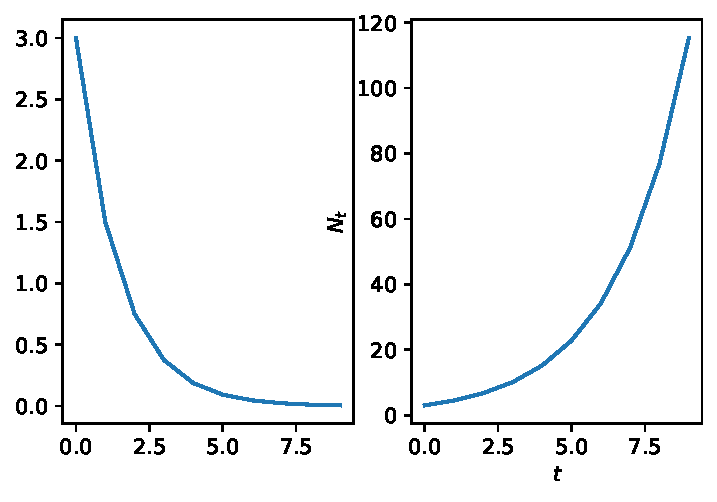
\includegraphics{MA32009-SinglePopDiscreteTimea_files/figure-pdf/fig-plotmalthusian-output-1.pdf}

}

\caption{\label{fig-plotmalthusian}A plot of the Malthusian model
solution when (a) \(r\)=0.5 and (b) \(r\)=1.5.}

\end{figure}

Can you describe the behaviour of the Malthusian model? How does it
depend on the value of the parameter \(r\)?

Qualitative analyses allows us to categorise solution behaviours into
different cases. For example, note that the behaviour of the population
at large \(t\) is governed by the magnitude of the parameter \(r\).

As \(t\rightarrow \infty\)

\[
 N \rightarrow 
\left\{
\begin{array}{ll}
\infty & r>1  \\
N_0& r=1  \\  
0 & r<1.     
\end{array} \right.
\]

In Figure~\ref{fig-plotmalthusian} solutions in each of the (nontrivial)
parameter regimes are plotted. When \(r<1\) the population tends to zero
and when \(r>1\) the population explodes.

Whilst the simplicity of the Malthusian model allows us to calculate
explicit solutions that yield insight into how the processes of birth
and death combine to give either net growth or net reduction in
population size, an obvious flaw with this model is that it displays
unbounded growth for \(r>1\). In most biological systems, other effects,
such as competition for resources or predation, will tend to limit a
population's size. In single species population models, these effects
are accounted for phenomenologically by introducing nonlinear terms into
the function \(f\).

\hypertarget{a-motivating-example-of-a-nonlinear-model---the-ricker-model}{%
\section{A motivating example of a nonlinear model - The Ricker
model}\label{a-motivating-example-of-a-nonlinear-model---the-ricker-model}}

Many models of population dynamics in discrete time were initially
developed to study fisheries. Well-studied examples include the Beverton
Holt model \[
N_{t+1}=\frac{rN_t}{1+\frac{N_t}{K}},
\] the Hassell model \[
N_{t+1}=\frac{rN_t}{(1+\frac{N_t}{K})^b},
\] and the Ricker model \[
N_{t+1}=N_te^{r(1-\frac{N_t}{K})}.
\] where \(r\), \(K\) and \(b\) are positive parameters. Below we
consider the Ricker model which was initially used to study Canadian
sockeye salmon population dynamics.

\hypertarget{model-development}{%
\subsection{Model development}\label{model-development}}

One way to capture a decreased growth rate at high densities, is to
assume that the per capita growth rate is an exponentially decreasing
function of population density, i.e.~ \[
f(N_t)=e^{r(1-\frac{N_t}{K})},
\] where \(r\) is a growth rate and \(K\) a carrying capacity (both
positive constants). Hence the governing equation is
\begin{equation}\protect\hypertarget{eq-RickerDefn1}{}{
N_{t+1}=N_te^{r(1-\frac{N_t}{K})}.
}\label{eq-RickerDefn1}\end{equation} Note that as the population size
gets large (\(N_t\gg K\)), the growth rate tends to zero but that for
small populations \(N_t\ll K\) the growth rate is approximately
constant. This is the Ricker model.

Note that the model is nonlinear and does not have an explicit solution.

\hypertarget{computational-solutions}{%
\subsection{Computational solutions}\label{computational-solutions}}

After directly computing numerical solutions of the Ricker model for
different values of the parameter \(r\), the data in
Figure~\ref{fig-plotricker} were obtained.

Note that model behaviour changes drastically as the parameter \(r\)
varies. For instance,

\begin{itemize}
\tightlist
\item
  when \(r=0.5\) (Figure~\ref{fig-plotricker} (a)), the solution
  monotonically approaches the value \(2\),
\item
  when \(r=1.5\) (Figure~\ref{fig-plotricker} (b)) it approaches two in
  an oscillatory manner; and
\item
  when \(r=2.5\) (Figure~\ref{fig-plotricker} (c)) it oscillates around
  two.
\end{itemize}

The above numerical results raise the following questions:

\begin{itemize}
\tightlist
\item
  can we develop tools that allow us to qualitatively describe how the
  model solutions depend on model parameters?
\item
  are the there certain families of solutions with qualitatively similar
  behaviours?
\item
  how do such families of solutions depend on model parameters?
\end{itemize}

We will return to analysis of the Ricker model in Worksheet 1.

\begin{figure}

{\centering 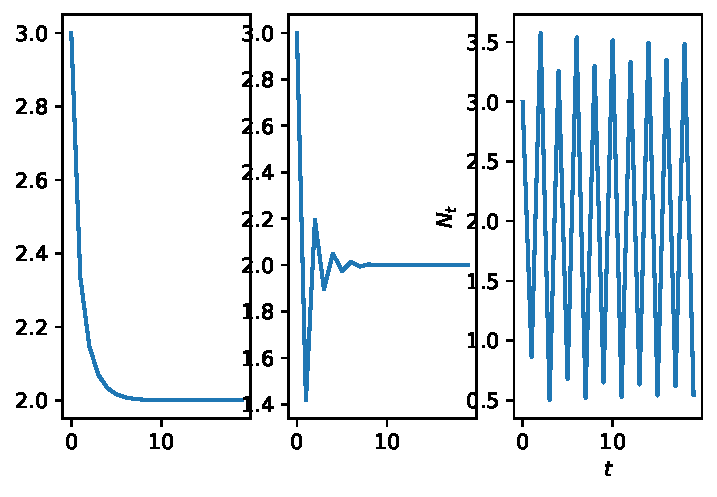
\includegraphics{MA32009-SinglePopDiscreteTimea_files/figure-pdf/fig-plotricker-output-1.pdf}

}

\caption{\label{fig-plotricker}A plot of numerical solutions of the
Ricker model. (a)r=0.5. (b) r=1.5. (c) r=2.5.}

\end{figure}

\hypertarget{general-techniques-for-analysing-nonlinear-difference-equations}{%
\section{General techniques for analysing nonlinear difference
equations}\label{general-techniques-for-analysing-nonlinear-difference-equations}}

In this section we develop techniques that will be used to analyse first
order, discrete-time models of the form
\begin{equation}\protect\hypertarget{eq-generaleqn}{}{ 
N_{t+1}=N_t f(N_t)=H(N_t).
}\label{eq-generaleqn}\end{equation}

\hypertarget{computational-solutions-1}{%
\subsection{Computational solutions}\label{computational-solutions-1}}

Perhaps the most obvious way to investigate an equation of the form of
Equation~\ref{eq-generaleqn} is to iteratively compute \(N_t\) over a
prescribed time range.

Hence given some initial population \(N_0\), the solution set
\(\{N_0,N_1,N_2,...,N_T\}\) is computed up to some end time \(T\). Such
an approach provides a numerical solution for a given parameter set and
initial condition. However, it does not provide much insight into the
general behaviour of model.

\hypertarget{fixed-points}{%
\subsection{Fixed points}\label{fixed-points}}

We define \(N^*\) to be a fixed point of Equation~\ref{eq-generaleqn} if
and only if \[ 
N^*=N^*f(N^*)=H(N^*).
\] Hence the fixed points can be identified by solving an algebraic
equation.

\hypertarget{linear-stability}{%
\subsection{Linear stability}\label{linear-stability}}

By linearising about the identified fixed points using a Taylor series
expansion, it can be determined whether or not small perturbations
around the fixed point grow or decay in subsequent iterations.

Making a change of dependent variables \[
N_t=N^*+\hat{N_t},
\] Equation~\ref{eq-generaleqn} transforms upon substitution to \[
 N^*+\hat{N}_{t+1} =  H(N^*+\hat{N}_t). 
\]

Taylor expanding the right-hand side yields \[
N^*+\hat{N}_{t+1}= H(N^*)+H'(N^*)\hat{N}_t + h.o.t. .
\]

Noting that at the fixed point \[
N^*= H(N^*), 
\] cancellation yields \[
\hat{N}_{t+1} = H'(N^*)\hat{N}_t + h.o.t. 
\] Hence considering only small perturbations about the fixed point, the
leading order behaviour of the perturbation is governed by \[
\hat{N}_{t} = (H'(N^*))^t\hat{N}_0.
\]

Hence the linear stability of the fixed point is governed by the sign
and magnitude of the term \(H'(N^*)\). If \[
 |H'(N^*)| >1,
\] the fixed point is unstable. Otherwise it it stable.

\hypertarget{cobwebbing-and-linear-stability}{%
\subsection{Cobwebbing and linear
stability}\label{cobwebbing-and-linear-stability}}

A cobweb diagram allows solutions of a first order difference equation
to be sketched without explicitly solving.

\hypertarget{an-algorithm-for-generating-a-cobweb-diagram}{%
\subsubsection{An algorithm for generating a cobweb
diagram}\label{an-algorithm-for-generating-a-cobweb-diagram}}

The cobweb diagram is created as follows:

\begin{itemize}
\tightlist
\item
  Plot the \(t^{th}\) iterate, \(N_t\), on the \(x\) axis and the
  \(t+1^{st}\), \(N_{t+1}\) on the \(y\) axis.
\item
  Sketch the net growth rate function \(H(N_t)\).
\item
  Sketch the line \(N_{t+1}=N_t\).
\item
  Note any intersections between the straight line and the graph of
  \(H(N_t)\) are fixed points.
\item
  Plot the first point \((N_0, H(N_0))\) on the cobweb diagram.
\item
  Plot a horizontal line between \((N_0, H(N_0))\) and
  \((H(N_0),H(N_0))\). Note \(N_1=H(N_0)\).
\item
  Plot a vertical line between \((N_1,N_1)\) and \((N_1,H(N_1))\).
  *Repeat steps 6 and 7.
\end{itemize}

Plotting cobweb diagrams in the vicinity of a fixed point \(N^*\) for
different values of \(H'(N^*)\) allows us to see graphically how the
derivative of the right-hand side affects linear stability of a fixed
point (see Figure~\ref{fig-cobwebstepbystep}). In particular,

\begin{itemize}
\tightlist
\item
  when \(H'(N^*)>1\), the fixed point is monotonically unstable;
\item
  when \(0<H'(N^*)<1\), the fixed point is monotonically stable;
\item
  when \(-1<H'(N^*)<0\), the fixed point is oscillatory stable;
\item
  when \(H'(N^*)=-1\), the fixed point is oscillatory; and
\item
  when \(H'(N^*)<-1\), the fixed point is oscillatory unstable.
\end{itemize}

\begin{figure}

{\centering 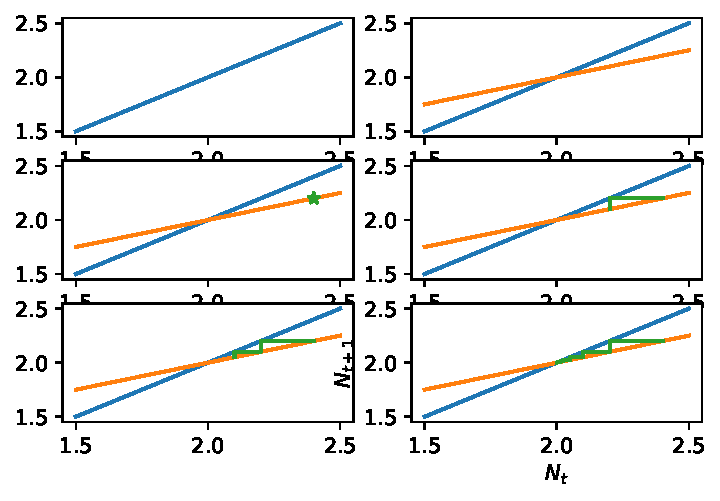
\includegraphics{MA32009-SinglePopDiscreteTimea_files/figure-pdf/fig-cobwebstepbystep-output-1.pdf}

}

\caption{\label{fig-cobwebstepbystep}Generating a cobweb plot.}

\end{figure}

\hypertarget{bifurcation-diagrams}{%
\subsection{Bifurcation diagrams}\label{bifurcation-diagrams}}

A bifurcation is a qualitative change in solution behaviour (either a
change in the number of fixed points or their stability). A bifurcation
diagram is a compact means of describing bifurcations as a function of
model parameters. Usually, the fixed point value of the population
(i.e.~\(N^*\)) is plotted against a model parameter of interest. From
this diagram one can immediately see how the number of fixed points and
their stability changes as a given parameter increases.

\hypertarget{perform-a-qualitative-analysis-on-the-matlhusian-model}{%
\subsection{Perform a qualitative analysis on the Matlhusian
model}\label{perform-a-qualitative-analysis-on-the-matlhusian-model}}

Let's work through the various concepts introduced above using the
Malthusian model (Equation~\ref{eq-MalthusianEqn}).

The fixed points satisfy \[
N^*=rN^*.
\] As \(r>0\) the only solution is \(N^*=0\).

In this case \[
H'(N_t)=r.
\] Hence the linear stability of the solution depends on the value of
the parameter \(r\) For \(r>1\) the fixed point \(N^*=0\) is
monotonically unstable. For \(r<1\) the fixed point \(N^*=0\) is
monotonically unstable. As expected this result is consistent with the
simulation results in Figure~\ref{fig-plotmalthusian}.

For cobweb diagram:

\begin{itemize}
\tightlist
\item
  Sketch axes and label with \(N_t\) and \(N_{t+1}\).
\item
  From linear stablity analysis note there are two qualitatively
  distinct cases (\(r<1\) and \(r>1\)). We will need a cobweb diagram
  for each case.
\item
  Case 1: graph the function \(H(N_t)\). In this case it is the straight
  line \(N_{t+1}=rN_t\) with \(r<1\).
\item
  Case 2: graph the function \(H(N_t)\). In this case it is the straight
  line \(N_{t+1}=rN_t\) with \(r>1\).
\item
  Fill in the cobwebbed trajectories with some arbitraily chosen initial
  condition.
\item
  Establish that behaviour of the cobweb is consistent with linear
  stability analysis.
\end{itemize}

\begin{figure}

{\centering 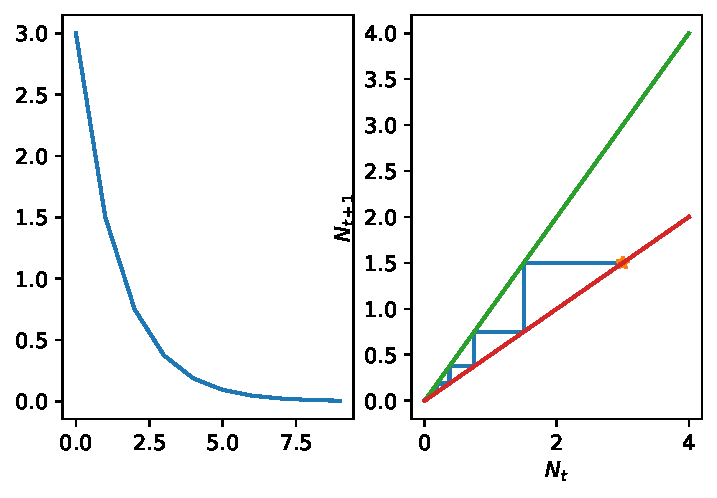
\includegraphics{MA32009-SinglePopDiscreteTimea_files/figure-pdf/fig-plotmalthusiancobweb-output-1.pdf}

}

\caption{\label{fig-plotmalthusiancobweb}A cobweb plot of the Malthusian
model solution when \(r\)=0.5. (a) Time series and (b) Cobweb diagrams.}

\end{figure}

For bifurcation diagram:

\begin{itemize}
\tightlist
\item
  We will plot the value of fixed point against a parameter of interest.
  In this case \(N^*\) against \(r\).
\item
  Deduce from fixed point and linear stability analysis whether there
  are any changes in solution behaviour as \(r\) varies (e.g.~number of
  solution or their linear stability).
\item
  In this case the value of the fixed point is independent of \(r\) but
  the the linear stability changes at \(r=1\). This is a bifurcation.
\item
  Use annotation to represent qualitative solution behaviour.
\end{itemize}

\hypertarget{a-nonlinear-model-of-population-dynamics-in-discrete-time}{%
\section{A nonlinear model of population dynamics in discrete
time}\label{a-nonlinear-model-of-population-dynamics-in-discrete-time}}

Consider a model of population growth given by
\begin{equation}\protect\hypertarget{eq-denslimgrowtheqn}{}{
N_{t+1}=\frac{\gamma N_t}{1+N_t^2},
}\label{eq-denslimgrowtheqn}\end{equation} where \(\gamma\in \Re^+\) is
the linear growth rate.

\hypertarget{the-per-capita-growth-rate}{%
\subsection{The per capita growth
rate}\label{the-per-capita-growth-rate}}

Note that the per capita growth rate is described by the function \[
f(N_{t})=\frac{\gamma}{1+N_t^2}.
\] Hence at large populations the per capita growth rate tends to zero
whilst for small populations it tends to \(\gamma\). Hence so long as
\(\gamma>1\) we will have net growth for small populations and net
removal for large populations. The net growth rate is given by \[
H(N_{t})=\frac{\gamma N_t}{1+N_t^2}.
\]

\hypertarget{numerical-solution}{%
\subsection{Numerical solution}\label{numerical-solution}}

In Figure~\ref{fig-plotdensmodel1} time series solution of the model are
plotted for parameter values \(\gamma=0.5\), \(\gamma=1.5\),
\(\gamma=2.5\). Note qualitative changes in model behaviour in the
different parameter regimes. Can you identify the fixed points? Are the
solutions oscillatory?

\begin{figure}

{\centering 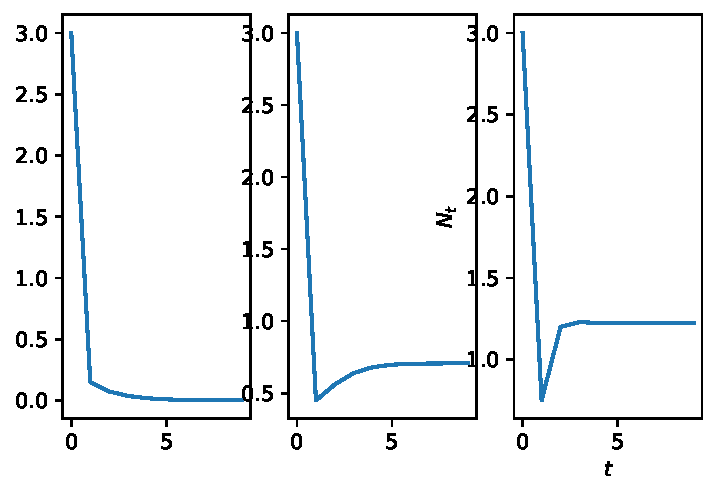
\includegraphics{MA32009-SinglePopDiscreteTimea_files/figure-pdf/fig-plotdensmodel1-output-1.pdf}

}

\caption{\label{fig-plotdensmodel1}Time series solution for (a)
\(g\)=0.5 and (b) \(g\)=1.5 and (c) \(g\)=10.5.}

\end{figure}

\hypertarget{fixed-points-1}{%
\subsection{Fixed points}\label{fixed-points-1}}

The fixed points of Equation~\ref{eq-denslimgrowtheqn} satisfy the
algebraic equation \[
N^*=\frac{\gamma N^*}{1+{N^*}^2}
\] which has solutions \[
N^* = 0  \ \ \ \ \textrm{and} \ \ \ \ N^*=\sqrt{\gamma-1}.
\]

\hypertarget{parameter-restrictions-for-biological-validity}{%
\subsubsection{Parameter restrictions for biological
validity}\label{parameter-restrictions-for-biological-validity}}

If \(\gamma<1\), there is only one biologically relevant fixed point. If
\(\gamma >1\) there are two fixed-points, \(N^*=0\) and
\(N^*=\sqrt{\gamma-1}\). Hence the value of the model parameter
\(\gamma\) qualitatively affects the behaviour and number of solutions.

\hypertarget{linear-stability-analysis}{%
\subsection{Linear stability analysis}\label{linear-stability-analysis}}

For the given model we compute \[
H'(N_t)= \frac{\gamma}{1+N_t^2} + \frac{-2 \gamma N_t^2}{(1+N_t^2)^2}.
\]

\hypertarget{n0}{%
\subsubsection{\texorpdfstring{\(N^*=0\)}{N\^{}*=0}}\label{n0}}

The stability of the fixed point \(N^*=0\) is determined by \[
H'(0)= \gamma.
\] Hence if \$ \gamma \textless1\$ the first fixed point is
monotonically stable as \(0<H'(0) < 1\).

When \(\gamma > 1\) the second fixed point becomes biologically relevant
and the first fixed point becomes monotonically unstable.

\hypertarget{nsqrtgamma-1}{%
\subsubsection{\texorpdfstring{\(N^*=\sqrt{\gamma-1}\)}{N\^{}*=\textbackslash sqrt\{\textbackslash gamma-1\}}}\label{nsqrtgamma-1}}

The stability of the second fixed point, \(N^*=\sqrt{\gamma-1}\), is
determined by

\[
\begin{aligned}
H'(\sqrt{\gamma-1})&= \frac{\gamma}{1+\gamma-1} + \frac{-2 \gamma (\gamma-1)}{(1+(\gamma-1))^2}, \\
&= \frac{2}{\gamma}-1.
\end{aligned}
\]

Hence if \(N^*\) were monotonically unstable,

\[
H'(\sqrt{\gamma-1}) = \frac{2}{\gamma}-1 >1,
\] and \[
\gamma<1.
\] As a necessary condition for the biological relevance of \(N^*\) is
that \(\gamma>1\) we obtain a contradiction. Hence \(N^*\), if it is
biologically relevant, cannot be monotonically unstable.

Suppose \(N^*\) is monotonically stable. Then \[
0<H'(N^*) <1 
\] which upon substitution yields \[
0<\frac{2}{\gamma}-1  <1. 
\] Hence \(1<\gamma<2\). Suppose \(N^*\) is oscillatory stable. Then \[
-1<H'(N^*) <0 
\] which upon substitution yields \[
-1<\frac{2}{\gamma}-1  < 0.
\] Hence \(\gamma>2\). Hence the linear stability of the fixed point
\(N^*=\sqrt{\gamma-1}\) depends on whether \(\gamma\) lies in the range
\([0,1]\), \([1,2 ]\) or \([2,\infty]\).

\hypertarget{cobweb-diagrams}{%
\subsection{Cobweb diagrams}\label{cobweb-diagrams}}

In Figure~\ref{fig-densmodelcobweb} cobweb diagrams illustrate model
behaviour in the three different parameter regimes. Note that the cobweb
diagrams can be sketched by hand, given an accurate enough sketch of the
right-hand side function \(H(N_t)\). Note also that the cobweb diagrams
are consistent with the linear stability analysis but that the linear
approximation is only valid close to the equilibrium point.

\begin{figure}

{\centering 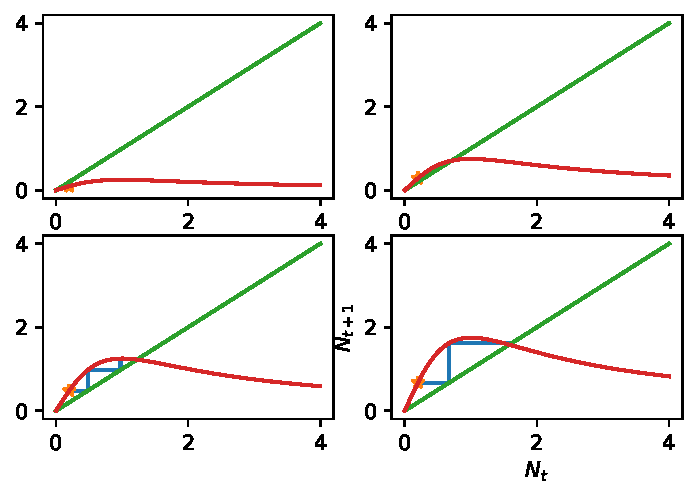
\includegraphics{MA32009-SinglePopDiscreteTimea_files/figure-pdf/fig-densmodelcobweb-output-1.pdf}

}

\caption{\label{fig-densmodelcobweb}Cobweb diagrams for different values
of gamma.}

\end{figure}

\hypertarget{bifurcation-diagram}{%
\subsection{Bifurcation diagram}\label{bifurcation-diagram}}

Bifurcations at the critical values \(\gamma=1\) and \(\gamma=2\) are
highlighted in the bifurcation diagram presented in
Figure~\ref{fig-densmodelbfc}. Note that the bifurcation diagram allows
classification of the different model behaviours in a single plot
without explicitly calculating the solution to the model.

\hypertarget{symbolic-computation}{%
\subsection{Symbolic computation}\label{symbolic-computation}}

We can use symbolic calculators to aid many of computations performed
above. Below is an example using the Python library sympi.

\begin{figure}

{\centering 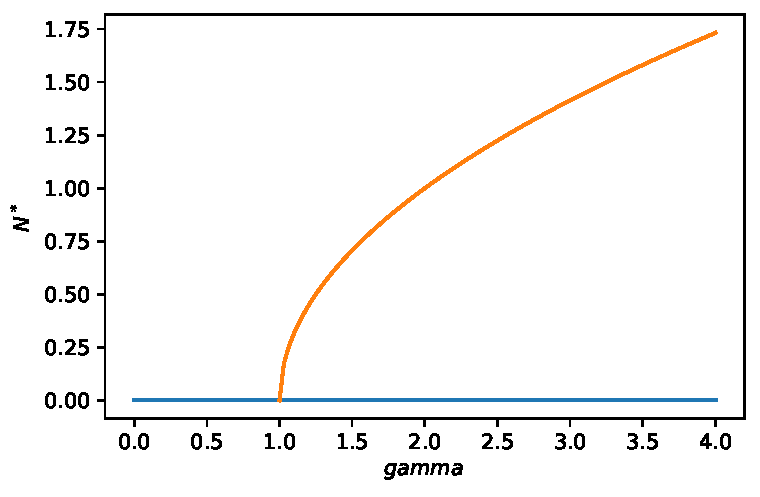
\includegraphics{MA32009-SinglePopDiscreteTimea_files/figure-pdf/fig-densmodelbfc-output-1.pdf}

}

\caption{\label{fig-densmodelbfc}A bifiurcation diagram.}

\end{figure}

Many of the calculations can be aided by using a symbolic calculator.

\hypertarget{code-calc1}{}
\begin{verbatim}
The FPs are:
[{N: 0}, {N: -sqrt(gamma - 1)}, {N: sqrt(gamma - 1)}]
The derivative of H is:
gamma*(1 - N**2)/(N**2 + 1)**2
The derivative evaluated at FP 1 is:
gamma
The derivative evaluated at FP 2 is:
(2 - gamma)/gamma
\end{verbatim}

\hypertarget{an-application---how-much-harvesting-can-a-population-sustain}{%
\section{An application - how much harvesting can a population
sustain?}\label{an-application---how-much-harvesting-can-a-population-sustain}}

Models of population dynamics can be used to study how interventions
will affect population dynamics. Extending from the model developed in
the previous example, a valid question might be what is the maximal rate
of harvesting a fish stock can sustain without becoming extinct? \#\#\#
Including a harvesting term Introducing a harvesting term at per capita
harvesting rate \(h\), the governing model equation becomes
\begin{equation}\protect\hypertarget{eq-harvestingmodel}{}{
N_{t+1}=\frac{\gamma N_t}{1+N_t^2} - h N_t,
}\label{eq-harvestingmodel}\end{equation}

and the questions we want to ask are: (i) does the introduction of
harvesting change the dynamics of the system?; and (ii) what rate of
harvesting such a population could withstand?

\hypertarget{direct-simulation}{%
\subsection{Direct simulation}\label{direct-simulation}}

Based on the previous analysis we consider the system in a parameter
regime where without harvesting there is a stable fixed point
(\(\gamma>1\)).

\begin{figure}

{\centering 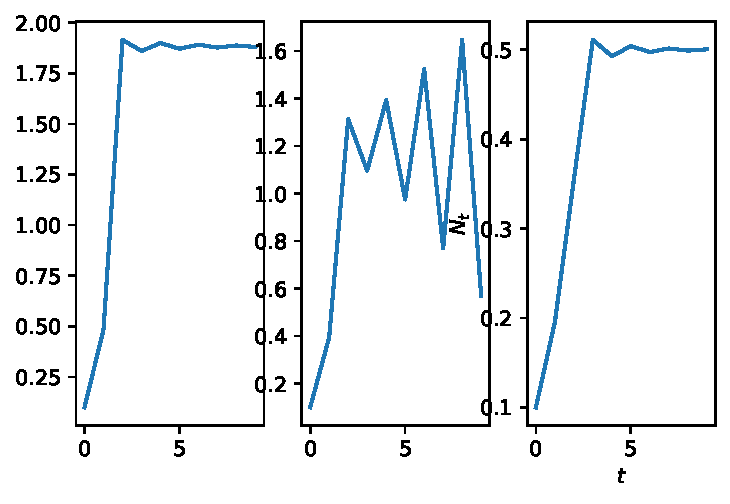
\includegraphics{MA32009-SinglePopDiscreteTimea_files/figure-pdf/fig-plotdensmodelharvest-output-1.pdf}

}

\caption{\label{fig-plotdensmodelharvest}Time series solution for (a)
\(g\)=0.5 and (b) \(g\)=1.5 and (c) \(g\)=10.5.}

\end{figure}

In Figure~\ref{fig-plotdensmodelharvest} time series solutions at
increasing harvesting rates (\(h=0.1\), \(h=1\), \(h=3\)) are presented.
For low harvesting rates the system behaves almost identically to the no
harvesting case but with an expected reduction in the fixed point value.
However for intermediate harvesting the population undergoes
oscillations. However, for further increased harvesting rates there
appears again to be a stable fixed point.

Can analysis of the model help us understand how/why changes in
solutions occur?

\hypertarget{fixed-points-2}{%
\subsection{Fixed points}\label{fixed-points-2}}

The fixed points of the system satisfy \[
N^*=\frac{\gamma N^*}{1+{N^*}^2} - h N^*.
\]

Hence the fixed points are \[
N^*=0
\]

and \[
N^*=\sqrt{\frac{\gamma}{1+h}-1}.
\]

Note that harvesting lowers the population size of the non-zero fixed
point (when it exists).

Can we deduce a condition that must hold on the parameters \(\gamma\)
and \(h\) in order that there is a non trivial biologically relevant
fixed point?

Requiring \[
N^* >0
\]

implies \[
\frac{\gamma}{1+h}-1>0.
\]

\hypertarget{linear-stability-1}{%
\subsection{Linear stability}\label{linear-stability-1}}

The linear stability is determined by \[
H'(N_t)=\frac{\gamma }{1+{N_t}^2} - \frac{2\gamma N_t^2 }{(1+{N_t}^2)^2} - h.
\]

At \(N^*=0\) we obtain \[
H'(0)=\gamma-h.
\]

Hence if \(\gamma>1+h\), \(N^*=0\) is unstable. Note that this is the
condition that determines whether the non-zero fixed point exists or
not.

At \[
N^*=\sqrt{\frac{\gamma}{1+h}-1},
\]

\[
H'\left(\sqrt{\frac{\gamma}{1+h}-1}\right)=\frac{\gamma }{1+\frac{\gamma}{1+h}-1} - \frac{2\gamma \frac{\gamma}{1+h}-1 }{(1+\frac{\gamma}{1+h}-1)^2} - h.
\]

Hence linear stability is a function of two parameters \(\gamma\) and
\(h\).

We can show that\\
\begin{equation}\protect\hypertarget{eq-arvestingH_prime}{}{
H'(N^*) = h^2\frac{2}{\gamma} + h\frac{2}{\gamma}(2-\gamma) + \frac{2}{\gamma}-1,
}\label{eq-arvestingH_prime}\end{equation}

and hence that when \(h=0\) we retrieve the stability condition from the
previous model.

\begin{figure}

{\centering 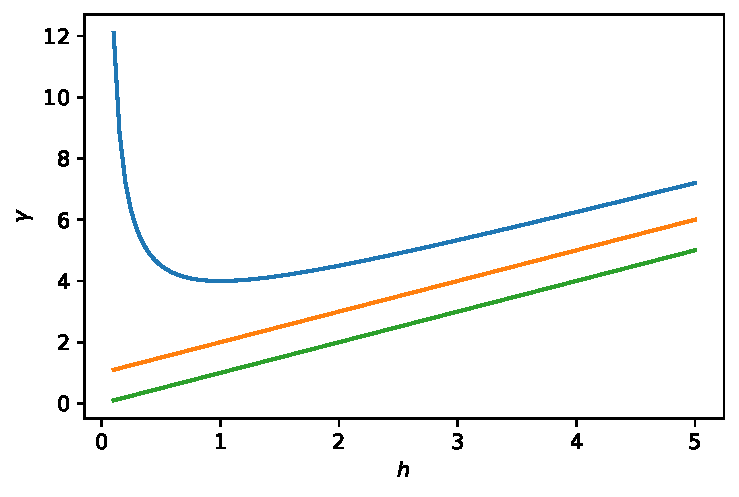
\includegraphics{MA32009-SinglePopDiscreteTimea_files/figure-pdf/fig-plotdensmodelharveststab-output-1.pdf}

}

\caption{\label{fig-plotdensmodelharveststab}Stability regions for the
harvesting model.}

\end{figure}

\hypertarget{stability-boundaries-in-the-hgamma-plane}{%
\subsection{\texorpdfstring{Stability boundaries in the \(h\gamma\)
plane}{Stability boundaries in the h\textbackslash gamma plane}}\label{stability-boundaries-in-the-hgamma-plane}}

The contour at \(H'(N^*)=1\) can be identified by solving \[
 h^2\frac{2}{\gamma} + h\frac{2}{\gamma}(2-\gamma) + \frac{2}{\gamma}-1 = 1,
\] yielding \[
 \gamma= 1+h.
\]

The contour at \(H'(N^*)=-1\) can be represented by \[
 h^2\frac{2}{\gamma} + h\frac{2}{\gamma}(2-\gamma) + \frac{2}{\gamma}-1 = -1,
\]

Solving for \(\gamma\) yields \[
\gamma=\frac{(1+h)^2}{h}.
\]

In Figure Figure~\ref{fig-plotdensmodelharveststab} we plot the contours
of the hypersurface \(H'(N^*)\) at the critical values of \(-1\), \(0\)
and 1. Note that the points in parameter space used to generate the
simulation results in Figure~\ref{fig-plotdensmodelharvest} are
\((h,\gamma)=(0.1,5)\) \((h,\gamma)=(1,5)\) and \((h,\gamma)=(3,5)\).
Cobweb diagrams in different regions of parameter space are presented in
Figure~\ref{fig-densharvestingmodelcobweb}. The plot in
Figure~\ref{fig-plotdensmodelharveststab} can be used to explain why the
model transfers from a stable fixed point, through oscillatory fixed
point and back to a stable fixed point as the harvesting rate increases
from 0.1, to \(1\) and then 5?

\begin{figure}

{\centering 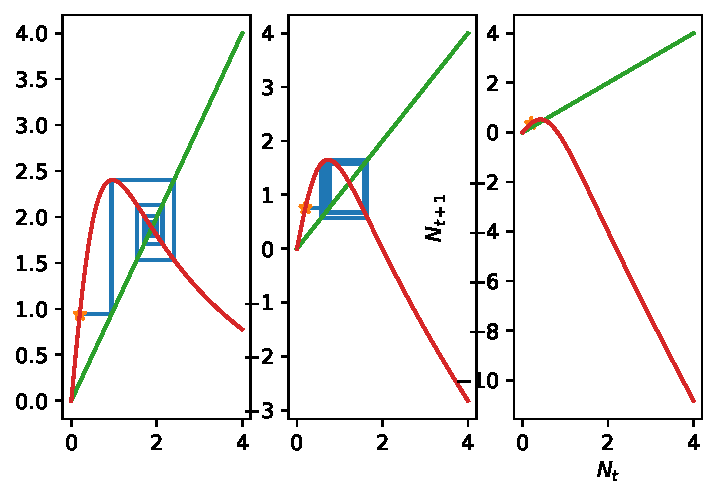
\includegraphics{MA32009-SinglePopDiscreteTimea_files/figure-pdf/fig-densharvestingmodelcobweb-output-1.pdf}

}

\caption{\label{fig-densharvestingmodelcobweb}Cobweb diagrams for
different values of h.}

\end{figure}

We can construct a cobweb diagram for the case \((h,\gamma)=(3,5)\).

Many of the above calculations can be aided using a symbolic calculator:

\hypertarget{code-calc1harvesting}{}
\begin{verbatim}
The FPs are:
{N: 0}
{N: -sqrt(gamma - h - 1)/sqrt(h + 1)}
{N: sqrt(gamma - h - 1)/sqrt(h + 1)}
The derivative of H is:
-N**2*gamma/(N**2 + 1)**2 + gamma/(N**2 + 1)**2 - h
The derivative evaluated at FP 0 is:
gamma - h
The derivative evaluated at FP 2 is:
(gamma + 2*(h + 1)*(-gamma + h + 1))/gamma
\end{verbatim}

\hypertarget{oscillations}{%
\section{Oscillations}\label{oscillations}}

Linear stability analysis describes the evolution of small perturbations
close to a fixed point. But far from a fixed point the nonlinear terms
that were dropped in a Taylor expansion are no longer negligible. In
particular, in the case where \(H'(N^*)<-1\), it can be the case that
regions of parameter space in which a fixed point is oscillatory
unstable can give rise to periodic and chaotic solutions.\\
\#\#\# Defining a periodic solution Consider the general form
\begin{equation}\protect\hypertarget{eq-genformagain}{}{
N_{t+1}=H(N_t)
}\label{eq-genformagain}\end{equation} A solution to
Equation~\ref{eq-genformagain} isdefined to be periodic with period
\(T\) if

\[
\begin{aligned}
N_{t+T}&=N_t \ \  \forall t, 
N_{t+\tau}&\neq N_t  \ \ \forall t, \  \ \ \tau<T.
\end{aligned}
\]

Period 2 solutions can be identified by looking for solutions that
repeat after two iterations. Suppose \(\bar{N}\) is a period 2 solution
of Equation~\ref{eq-genformagain} and let \(\bar{N}=N_1\). Then \[
N_{2}=H(\bar{N}).
\] However, \[
N_{3}=H(N_2)=H(H(\bar{N}))
\] and if \(\bar{N}\) is a period 2 solution \(N_3=N_1=\bar{N}\). Hence
period 2 solutions can be calculated by solving the algebraic equation
\[
\bar{N}=H(H(\bar{N})).
\] Note that period two solutions are fixed points of the problem \[
N_{t+2}=H^2(N_t)=g(N_t).
\] Using the tools we have developed, period solutions and their
stability can be determined. Furthermore, longer period solutions can be
identified by generalising the argument but at the expense of ever
increasingly complicated right-hand side functions. In many systems,
such as the harvesting model and the logistic equation, increasing the
growth rate parameter leads initially to the fixed point becoming
unstable and the emergence of period two solutions, then period 4
solutions and so on until eventually there is a transition to chaotic
solutions (see, for example,
Figure~\ref{fig-densharvestingmodelcobwebp4}).

\begin{figure}

{\centering 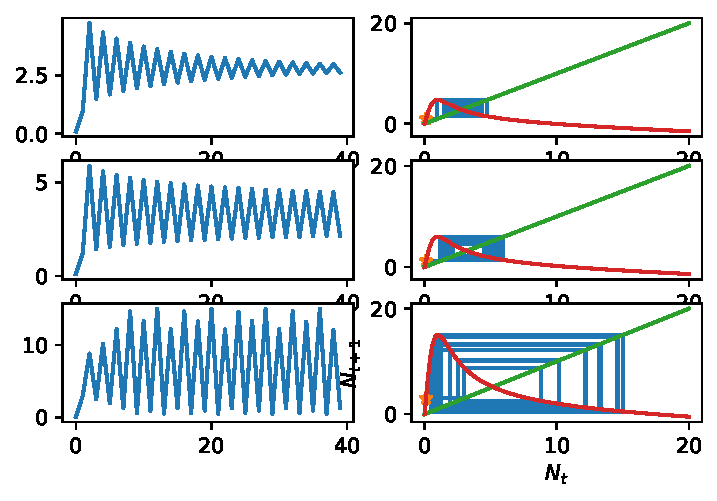
\includegraphics{MA32009-SinglePopDiscreteTimea_files/figure-pdf/fig-densharvestingmodelcobwebp4-output-1.pdf}

}

\caption{\label{fig-densharvestingmodelcobwebp4}Transition form period 2
to period 4 solutions in the harvesting model}

\end{figure}

Exercise: identify an equation satisfied by period 2 solutions of the
logistic map \[ 
 N_{t+1}=rN_1(1-N_t).
\]

\hypertarget{a-note-on-the-modelling-of-real-world-fish-stocks}{%
\section{A note on the modelling of real-world fish
stocks}\label{a-note-on-the-modelling-of-real-world-fish-stocks}}

You can find reports on fish stocks (measurements and modelling work)
from the International Council for the Exploration of the Sea at the
\href{http://www.ices.dk/Pages/default.aspx}{link}. Here's a link to the
data for \href{https://tinyurl.com/ya8sh72j}{Atlantic salmon}. Note that
although the models we have worked on are not detailed enough to
accurately model real fish population dynamics, many of the principles
we have covered arise in the cutting edge models.

\hypertarget{multi-species-population-dynamics}{%
\chapter{Multi species population
dynamics}\label{multi-species-population-dynamics}}

\hypertarget{multiple-species-in-discrete-time}{%
\chapter{Multiple species in discrete
time}\label{multiple-species-in-discrete-time}}

In this chapter we generalise the previous approach by considering the
population dynamics of two interacting populations.

\hypertarget{a-general-model-of-two-interacting-species-in-discrete-time}{%
\section{A general model of two interacting species in discrete
time}\label{a-general-model-of-two-interacting-species-in-discrete-time}}

Let \(N_t\) and \(P_t\) represent population densities at time \(t\)
where \(t\) is a discrete variable.

We consider governing equations of the form
\begin{equation}\protect\hypertarget{eq-discretetimetwovar}{}{
\begin{aligned}
N_{t+1}=f(N_t,P_t), \nonumber \\
P_{t+1}=g(N_t,P_t).
\end{aligned}
}\label{eq-discretetimetwovar}\end{equation} where the population
dynamics of the species are coupled to one another via the functions
\(f\) and \(g\).

The precise form for \(f\) and \(g\) will be defined by the biological
system under study. Typical interpopulation interactions that are
studied are: predator prey models, competition and cooperation.

\hypertarget{general-techniques-for-analysing-coupled-first-order-difference-equations}{%
\section{General techniques for analysing coupled first order difference
equations}\label{general-techniques-for-analysing-coupled-first-order-difference-equations}}

\hypertarget{fixed-points-3}{%
\subsection{Fixed points}\label{fixed-points-3}}

The fixed points of Equation~\ref{eq-discretetimetwovar} \((N^*,P^*)\)
satisfy \[
\begin{aligned}
N^*=g(N^*,P^*) \nonumber \\
P^*=f(N^*,P^*).
\end{aligned}
\]

\hypertarget{linear-stability-analysis-1}{%
\subsection{Linear stability
analysis}\label{linear-stability-analysis-1}}

To consider linear stability of a steady state we consider the change of
variable \[
\begin{aligned}
N_t&=N^*+\hat{N}_{t},   \nonumber\\
P_t&=P^*+\hat{P}_{t}.  \nonumber
\end{aligned}
\] After substitution in Equation~\ref{eq-discretetimetwovar} and making
Taylor expansions about \((N^*,P^*)\) we obtain at leading order

\begin{equation}\protect\hypertarget{eq-discretetimesecondorderdiff}{}{
\left(\begin{array}{c}
\hat{N}_{t+1} \\ \hat{P}_{t+1}\end{array}\right) = \left(\begin{array}{rr}
\frac{\partial f}{\partial N}&\frac{\partial f}{\partial P} \\ \frac{\partial g}{\partial N }&\frac{\partial g}{\partial P} \end{array}\right)_{(N^*,P^*)} \left(\begin{array}{c} \hat{N}_{t} \\ \hat{P}_{t}\end{array}\right).
}\label{eq-discretetimesecondorderdiff}\end{equation}

Note the appearance of the Jacobian matrix \[
A= \left(\begin{array}{rr}
\frac{\partial f}{\partial N}&\frac{\partial f}{\partial P} \\ \frac{\partial g}{\partial N }&\frac{\partial g}{\partial P} \end{array}\right)_{(N^*,P^*)} \left(\begin{array}{c} \hat{N}_{t} \\ \hat{P}_{t}\end{array}\right).
\]

\hypertarget{solving-the-linearised-problem}{%
\subsection{Solving the linearised
problem}\label{solving-the-linearised-problem}}

Defining \[
\mathbf{w}_t=\left(\begin{array}{c}\hat{N}_{t} \\ \hat{P}_{t}\end{array}\right), 
\]

\[
\mathbf{w}_{t+1}=A\mathbf{w}_{t}
\] By solving this linear system we can investigate whether small
perturbation about the fixed point grow or decay in magnitude as time
evolves and hence determine the linear stability of the fixed point.

The solution of Equation~\ref{eq-discretetimesecondorderdiff} takes the
form \[
\mathbf{w}_t=\sum_{i=1}^2 C_i \lambda_i^t\mathbf{c}_i,
\] where the \(C_i\)'s are constants determined by initial conditions
and the \(\lambda_i\)'s and \(\mathbf{c}_i\)'s are the eigenvalues and
eigenvectors of A, respectively. From this form we can see that if the
magnitude of all eigenvalues is less than one, i.e. \[
|\lambda_i|<1, \ \ \ \ \ \forall i,
\] the fixed point is linearly stable. If at least one of the
eigenvalues has \(|\lambda_i|>1\) then the fixed point is unstable to
linear perturbations.

\hypertarget{jury-conditions}{%
\subsection{Jury conditions}\label{jury-conditions}}

In many cases it is not very useful to explicitly compute the
eigenvalues of the Jacobian matrix. In such cases we can employ the Jury
conditions in order to determine when a fixed point is linearly stable.

Recall that for a two dimensional matrix, the eigenvalues satisfy the
quadratic characteristic equation

\[
\lambda^2- trA \lambda + detA=0.
\]

The stability of the fixed is guaranteed if \(|\lambda _i|<1\)
\(\forall i\).

Consider the characteristic equation \[
P(\lambda)=\lambda^2 + a \lambda +b=0,
\] where \(a,b \in \Re\). Note that \(a=-tr{A}\) and \(b=\det{A}\).

The Jury conditions state that \(|\lambda_i |<1 \forall \ \  i\) if, and
only if, * \(b<1\), * \(1+a+b>0\), * *\(1-a+b>0\). See
Figure~\ref{fig-juryconditions} for schematic diagram.

\begin{figure}

{\centering 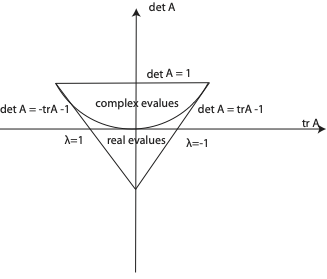
\includegraphics{JuryConditions2D.png}

}

\caption{\label{fig-juryconditions}Jury conditions}

\end{figure}

\hypertarget{proof-of-the-jury-conditions}{%
\subsection{Proof of the Jury
conditions}\label{proof-of-the-jury-conditions}}

The roots of \(P(\lambda)\) are \[
\lambda_{1,2}=\frac{-a \pm \sqrt{a^2-4b}}{2}.
\]

\hypertarget{complex-roots}{%
\subsection{Complex roots}\label{complex-roots}}

Suppose \(a^2-4b< 0\). The roots are complex. Since \(b\) is equal to
the product of the roots, we find that

\[
b=\lambda_1\lambda_2 = |\lambda_1|^2 = |\lambda_2^2|.
\] Hence \(\lambda_i<1\) \(\forall \ \ i\) if and only if \(b<1\).

For the other conditions we introduce the identity: \[
a^2-4b=(|a|-2)^2 - 4(1+b-|a|).
\] Therefore, when \(a^2-4b<0\), the inequality requires \[
(|a|-2)^2 - 4(1+b-|a|)<0.
\] This can only occur if \[
1+b-|a| >0 \implies 1+b-a>0 \ \ \textrm{and} \ \  1+b+a>0.
\]

\hypertarget{real-roots}{%
\subsection{Real roots}\label{real-roots}}

Suppose \(a^2-4b\geq 0\)

The largest magnitude of the roots is \[
R=\max\{|\lambda_1|,|\lambda_2|\} =  \frac{|a| + \sqrt{a^2-4b}}{2}.
\] This is an increasing function of \(|a|\).

\(R=1\) \[
\implies  \frac{|a| + \sqrt{a^2-4b}}{2}=1
\implies |a|-2=-\sqrt{|a|^2-4b}
\implies |a|^2-4|a|+4=|a|^2-4b 
\implies |a|=b+1.
\] Hence \(0\leq R < 1\) if and only if \(0\leq |a|<1+b\). Also, since
\(|\lambda_i|<1 \forall i\) implies that \(|\lambda_1\lambda_2|<1\), it
follows that \(|b|<1\) must hold.

\hypertarget{host-parasitoid-infection}{%
\section{Host Parasitoid infection}\label{host-parasitoid-infection}}

Parasitoids are creatures that have a free living and parasitic stage.
The free-living adult lays eggs in a host that later hatch and develop
after eating the host. The discrete stages of the parasitoids life cycle
and the dependence on its reproduction on the availability of host
suggest a discrete time, multi species models. Let \(N_{t}\) and \(P_t\)
represent the number of hosts and parasitoids at time \(t\),
respectively. Let \(R_0\) represent the reproductive ratio of host in
the absence of parasites and \(C\) the average number of viable eggs
laid by each parasite on a host. \#\#\# Model equations

We consider equations of the form
\begin{equation}\protect\hypertarget{eq-discretetimetwovar}{}{
\begin{aligned}
N_{t+1}&=R_0N_t f(N_t,P_t), \nonumber \\
P_{t+1}&=CN_t (1- f(N_t,P_t)). \nonumber
\end{aligned}
}\label{eq-discretetimetwovar}\end{equation}

The justification for this form is that at a given time \(t\) there are
\(N_t\) hosts. A total of \(N_t f(N_t,P_t)\) escape the parasite and are
able to reproduce whilst a total of \(N_t(1-f(N_t,P_t))\) do not escape
the parasite and lead to parasitic reproduction at the next time step.

Choosing \[
f(N_t,P_t)=e^{-aP_t},
\] yields the Nicholson Bailey model
\begin{equation}\protect\hypertarget{eq-nichbail}{}{
\begin{aligned}
N_{t+1}=R_0N_t e^{-aP_t}, \nonumber \\
P_{t+1}=CN_t (1- e^{-aP_t}). 
\end{aligned}
}\label{eq-nichbail}\end{equation}

\hypertarget{numerical-solution-1}{%
\subsection{Numerical solution}\label{numerical-solution-1}}

\begin{figure}

{\centering 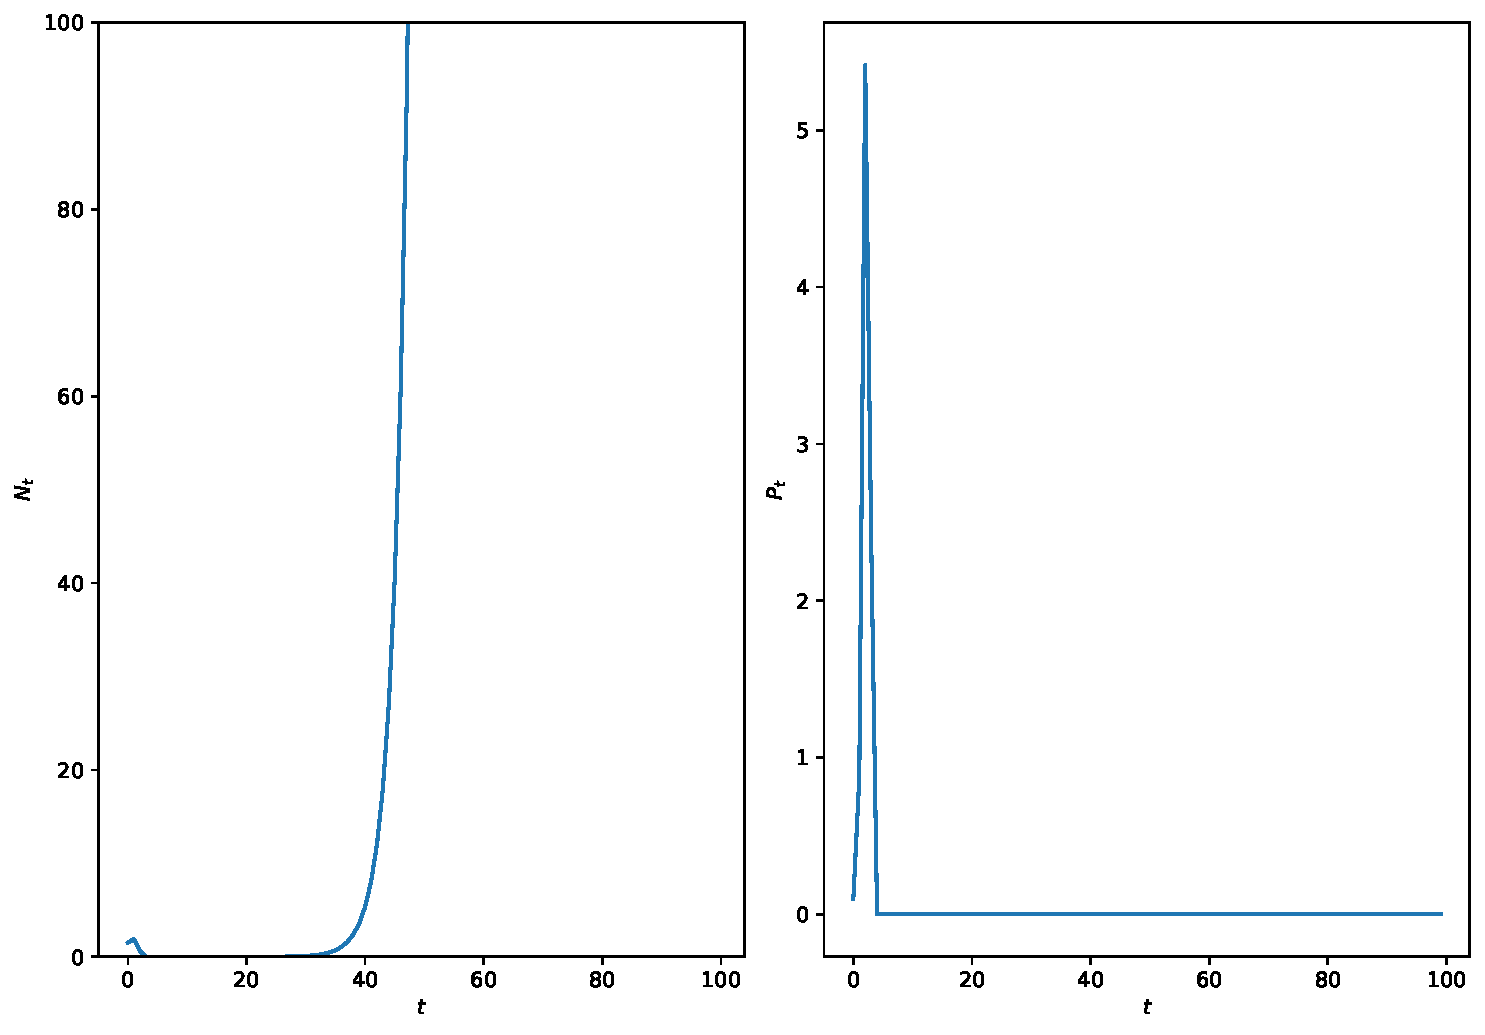
\includegraphics{DiscreteModels2d_files/figure-pdf/fig-plotnicolsonbailey-output-1.pdf}

}

\caption{\label{fig-plotnicolsonbailey}A plot of the Nicholson Bailey
model solution.}

\end{figure}

\hypertarget{fixed-points-4}{%
\subsection{Fixed points}\label{fixed-points-4}}

The fixed points satisfy \[
\begin{aligned}
N^*=R_0N^*e^{-aP^*}, \nonumber \\
P^*=CN^* (1- e^{-aP^*}). 
\end{aligned}
\]

The first equation yields \[
N^*=0.
\]

Suppose \(N^*\neq 0\) \[
1=R_0e^{-aP^*}.
\]

Hence \[
P^*=\frac{1}{a}\ln R_0.
\]

Consider the second equation. Suppose \(N^*=0\). We obtain \[
P^*=0. 
\] Hence one fixed point is \((0,0)\).

Suppose \(P^*=\frac{1}{a}\ln R_0\). \[
\frac{1}{a}\ln R_0 = CN^*(1-\frac{1}{R_0}).
\] Hence \[
N^* = \frac{\frac{1}{a}\ln R_0 }{C(1-\frac{1}{R_0})} = \frac{R_0\ln R_0 }{aC(R_0-1)}.
\] Hence the second fixed point is \[
\left(\frac{R_0\ln R_0 }{aC(R_0-1)},\frac{1}{a} \ln R_0 \right).
\]

We can verify by substitution that \[
\left(\frac{R_0\ln R_0 }{aC(R_0-1)},\frac{1}{a} \ln R_0 \right).
\] is a fixed point. We can then deduce a condition on the model
parameters that must hold in order that the fixed point is biologically
relevant.

To verify by substitution we substitute the proposed solution into the
governing equations. Note that \[
e^{-aP^*}=\frac{1}{R_0}.
\] In this case \begin{equation}\protect\hypertarget{eq-nichbail}{}{
\begin{aligned}
\frac{R_0\ln R_0 }{aC(R_0-1)}=R_0 \frac{R_0\ln R_0 }{aC(R_0-1)}\frac{1}{R_0}, \nonumber \\
\frac{1}{a} \ln R_0=C\frac{R_0\ln R_0 }{aC(R_0-1)} (1-\frac{1}{R_0}). 
\end{aligned}
}\label{eq-nichbail}\end{equation}

Cancellation shows that both equations hold. Hence the fixed point is a
valid fixed point. To be biologically relevant we require that both
components of the solution are real and positive. In this case this
leads to the condition \(R_0>1\)\}.

\hypertarget{linear-stability-2}{%
\subsection{Linear stability}\label{linear-stability-2}}

The Jacobian matrix is given by \[
A_{(N_t,P_t)}= \left(\begin{array}{cc}
R_0e^{-aP_t}&-R_0aN_te^{-aP_t} \\ c(1-e^{-aP_t})&aCN_te^{-aP_t} \end{array}\right).
\]

\hypertarget{linear-stability-of-the-trivial-fixed-point}{%
\subsection{Linear stability of the trivial fixed
point}\label{linear-stability-of-the-trivial-fixed-point}}

Evaluating at (0,0) yields \[
A= \left(\begin{array}{cc}
R_0 & 0 \\ 0 & 0 \end{array}\right).
\] Hence the eigenvalues are \(R_0\) and 0. If \(0<R_0<1\) (0,0) is
stable whilst if \(R_0>1\) (0,0) is unstable.

\hypertarget{linear-stability-of-the-nontrivial-fixed-point}{%
\subsection{Linear stability of the nontrivial fixed
point}\label{linear-stability-of-the-nontrivial-fixed-point}}

We can show that the Jacobian matrix evaluated at the nontrivial fixed
point can be written as \[
A= \left(\begin{array}{cc}
1&-\frac{R_0 \ln R_0}{c(R_0-1)} \\ c(1-\frac{1}{R_0})&\frac{\ln R_0}{R_0-1} \end{array}\right) .
\] and deduce that the eigenvalues of A satisfy the characteristic
polynomial \[
\lambda^2 - \lambda\left(1+\frac{\ln R_0}{R_0-1}\right)+ \frac{R_0\ln(R_0)}{R_0-1}=0.
\]

\hypertarget{employing-the-jury-conditions}{%
\subsection{Employing the Jury
conditions}\label{employing-the-jury-conditions}}

To proceed with linear stability analysis we employ the Jury conditions.
Consider the polynomial \[
\lambda^2+a\lambda+b=0,
\] In our case \[
a= - (1+\frac{\ln R_0}{R_0-1}) 
\] and \[
b=\frac{R_0\ln(R_0)}{R_0-1}.
\]

The third Jury condition (\(b<1\)) implies that for linear stability \[
\ln R_0 < 1-\frac{1}{R_0}.
\] To demonstrate that this inequality is not true for \(R_0>1\), let
\(f_1=\ln R_0\) and \(f_2=1- 1/R_0\). When \(R_0=1\), \(f_1=f_2=0\).
However, \[
f_1'=\frac{1}{R_0}  \ \ \textrm{and} \ \ f_2'=\frac{1}{R_0^2},
\] implies \[
f_1'>f_2'  \ \ \forall \ R_0>1.
\] Hence \[
\ln R_0 > 1-\frac{1}{R_0}.
\] Hence the fixed point is unstable if \(R_0>1\).

\part{Continuous time}

\hypertarget{single-species-population-dynamics-1}{%
\chapter{Single species population
dynamics}\label{single-species-population-dynamics-1}}

In this chapter we define time, \(t\), to be a continuous variable and
the population density, \(N(t)\), to represent the size of a given
population.

\hypertarget{the-malthusian-linear-model}{%
\section{The Malthusian (linear)
model}\label{the-malthusian-linear-model}}

\hypertarget{deriviation}{%
\subsection{Deriviation}\label{deriviation}}

As time is now a continuous variable, we consider an interval of time
\(\delta t\). Consider a population of size \(N(t)\). If the per capita
production rate is \(b\), then in time \(\delta t\) the increase in
population size will be \[
b N(t) \delta t.
\] Similarly, if the per capita death rate is \(d\), the decrease in
population size in time \(\delta t\) will be \[
d N(t) \delta t.
\] Hence \[
N(t+\delta t)= N(t) + (bN(t)-dN(t))\delta t.
\] Rearranging and taking the limit as \(\delta t \rightarrow 0\) yields
\[
\frac{dN}{dt}=(b-d)N=rN(t).
\]

\hypertarget{solution}{%
\subsection{Solution}\label{solution}}

The solution is given by \[
N(t)=N_0\exp(rt).
\]

We can describe qualitatively different solutions behaviours.

If \(r>0\) the solution increases exponentially with time. If \(r<0\) it
decreases exponentially. When \(r=0\) the solution is constant.

Malthusian growth in the continuous time model leads to either a
constant population, exponentially increasing or exponentially
decreasing growth. As was the case for the discrete time model, such a
model could account for biological system only in particularly limited
circumstances.

The Malthusian model (constant per capita growth rate) can exhibit a
limited range of behaviour. To account for limitation of population
growth at large population densities due to, for example, limited
resources, we consider nonlinear per capita growth rates.

\hypertarget{tools-for-analysing-the-dynamics-of-a-single-population-in-continuous-time}{%
\section{Tools for analysing the dynamics of a single population in
continuous
time}\label{tools-for-analysing-the-dynamics-of-a-single-population-in-continuous-time}}

Let \(N=N(t)\). We consider the general form for a single species model
defined in continuous time
\begin{equation}\protect\hypertarget{eq-gensinglespecodeagain}{}{
\frac{dN}{dt}=f(N)N=H(N),
}\label{eq-gensinglespecodeagain}\end{equation} where \(f\) is the per
capita growth rate and \(H\) is the net growth rate.

\hypertarget{numerical-solution-2}{%
\subsection{Numerical solution}\label{numerical-solution-2}}

Although an equation of the form Equation~\ref{eq-gensinglespecodeagain}
may not be explicitly integrable, so long as the right-hand side is
sufficiently well behaved, we can numerically integrate the problem
(e.g.~using packages such as Python's odeint). Such a technique provides
a numerical approximation to the exact solution, given specific values
of model parameters and initial conditions (i.e.~we can graph
solutions).

\hypertarget{nondimensionalisation}{%
\subsection{Nondimensionalisation}\label{nondimensionalisation}}

We nondimensionalise a model by changing from variables that have
dimensions (both dependent and independent) to variables that are
dimensionless.

\hypertarget{dimensional-analysis}{%
\subsubsection{Dimensional analysis}\label{dimensional-analysis}}

The dimensions/units of each term in a model must be consistent. This
observation helps to determine the units of different parameters in a
model.

For example, we can deduce that the units of the parameter \(r\) in the
Malthusian model \[
\frac{dN}{dt}=rN.
\]

The units of the left-hand term are \[
\frac{\# pop density}{\# time}.
\]

The units of the term on the right-hand side are \[
\#r\#popdensity.
\]

For dimensional consistency \[
\#r = \frac{1}{\#time}.
\]

\hypertarget{dimensionless-variables}{%
\subsubsection{Dimensionless variables}\label{dimensionless-variables}}

We could nondimensionalise Equation~\ref{eq-gensinglespecodeagain} by
defining the dimensionless variables \[
\begin{aligned}
n=\frac{N}{\tilde{N}} \nonumber \\
\tau=\frac{t}{\tilde{T}}.\nonumber
\end{aligned}
\]

Making the proposed change of variables in
Equation~\ref{eq-gensinglespecodeagain} we obtain the dimensionless
model \[
\frac{dn}{d\tau}= \frac{\tilde{T}}{\tilde{N}}H(\tilde{N}n(\tau)).
\] The choice for scalings is in general not unique (i.e.~\(N^*\) and
\(T^*\)). Appropriate choices can result in fewer dimensionless
parameters in the dimensionless model.

Exercise: Show that the Mathusian model \[
\frac{dN}{dt}=rN
\] can be written in nondimensional form \[
\frac{dn}{d\tau}=n.
\]

Introducing dimensionless variable \[
n=\frac{N}{\tilde{N}} \quad \tau=\frac{t}{\tilde{T}}
\] yields \[
\frac{dn}{d\tau}=r\tilde{T}n
\] Choosing \[
\tilde{T}=\frac{1}{r} 
\] yields \[
\frac{dn}{d\tau}=n.
\]

\hypertarget{steady-state}{%
\subsection{Steady-state}\label{steady-state}}

We denote steady-state solutions of
Equation~\ref{eq-gensinglespecodeagain} using \(N=N^*\). At a
steady-state, \[
\frac{dN}{dt}=0
\] and hence steady-states can be obtained by solving the algebraic
equation \[
H(N^*)=0.
\]

\hypertarget{linear-stability-analysis-2}{%
\subsection{Linear stability
analysis}\label{linear-stability-analysis-2}}

\hypertarget{a-change-of-dependent-variable}{%
\subsubsection{A change of dependent
variable}\label{a-change-of-dependent-variable}}

To perform a linear stability analysis we make the change of variables
\[
N(t)=N^*+\hat{N}(t)
\] where the new dependent variable, \(\hat{N}(t)\), is a perturbation
about the steady state.

The time derivative on the left-hand side of
Equation~\ref{eq-gensinglespecodeagain} transforms to \[
\frac{dN}{dt}= \frac{d }{dt} (N^*) + \frac{d }{dt}(\hat{N}(t))=\frac{d\hat{N}(t) }{dt}.
\] Hence Equation~\ref{eq-gensinglespecodeagain} transforms to \[
\frac{d\hat{N}(t) }{dt} = H(N^*+\hat{N}(t)).
\]

\hypertarget{taylor-expansion-and-a-linear-system}{%
\subsubsection{Taylor expansion and a linear
system}\label{taylor-expansion-and-a-linear-system}}

Employing the Taylor expansion on the right-hand side of
Equation~\ref{eq-gensinglespecodeagain} and making the assumption that
perturbations are small \[
\frac{d\hat{N}(t) }{dt} = H(N^*)+  H'(N^*)\hat{N}(t) + H''(N^*)\hat{N}^2(t) + h.o.t.
\] Noting that\\
\[
H(N^*)=0
\] and retaining linear terms yields \[
\frac{d\hat{N}(t) }{dt} =  H'(N^*)\hat{N}(t)
\] with solution \[
\hat{N}(t)=  \eta e^{H'(N^*) t}
\] where \(\eta\) is some initial perturbation about the steady-state.

\hypertarget{a-condition-for-linear-stability}{%
\subsubsection{A condition for linear
stability}\label{a-condition-for-linear-stability}}

When \(H'(N^*)>0\) the perturbation grows exponentially fast and the
steady-state is unstable. When \(H'(N^*)<0\) the perturbation decays
exponentially fast and the steady-state is stable.

\hypertarget{graphical-solution}{%
\subsection{Graphical solution}\label{graphical-solution}}

We can graphically identify steady-states and their stability by
plotting \(dN/dt\) against \(N(t)\). Steady-states arise at the roots of
\(H(N)\). The sign of the derivative at a root determines its linear
stability.

\hypertarget{bifurcation-diagrams-1}{%
\subsection{Bifurcation diagrams}\label{bifurcation-diagrams-1}}

Bifurcations arise when the number of solutions or their stability
changes at a given value of a model parameter. By plotting the steady
state solutions against a model parameter and using annotation to
represent stability of solutions we can obtain a bifurcation diagram.

As an exercise perform a qualitative analysis of the Malthusian model.

\hypertarget{the-logistic-growth-model}{%
\section{The logistic growth model}\label{the-logistic-growth-model}}

\hypertarget{model-development-1}{%
\subsection{Model development}\label{model-development-1}}

Let \(N=N(t)\). The logistic model, due to Verhulst, takes the form
\begin{equation}\protect\hypertarget{eq-logisticode}{}{
\frac{dN}{dt}=rN(t)\left (1-\frac{N(t)}{K}\right),
}\label{eq-logisticode}\end{equation}

where \(r\) is the linear growth rate and \(K\) is carrying capacity. We
consider both \(r,K\in \Re^+\).

Questions to ask of such a model are: what type of biologically
realistic solutions does it possess? Are there steady-states? If so, are
they stable or unstable? Are there bifurcations in solutions?

\hypertarget{numerical-solutions}{%
\subsubsection{Numerical solutions}\label{numerical-solutions}}

In Figure~\ref{fig-logisticgrowthmodel} we present numerical solutions
of equation using different initial conditions. Note the limiting
behaviour of solutions as \(t\rightarrow \infty\). In
Figure~\ref{fig-logisticgrowthmodel} it is clear that even though some
solutions are initialised at \(N_0=0.1\), much closer to \(N^*=0\) than
\(N^*=K\), they tend to the limit \(N=K\). Why do solutions not tend to
\(N^*=0\)?

\begin{figure}

{\centering 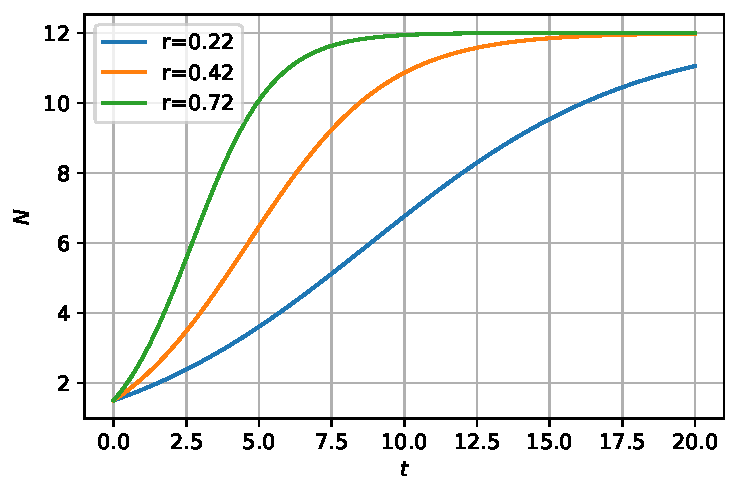
\includegraphics{SinglePopODEMOdels_files/figure-pdf/fig-logisticgrowthmodel-output-1.pdf}

}

\caption{\label{fig-logisticgrowthmodel}RHS of spr. budworm model}

\end{figure}

\hypertarget{dimensional-analysis-and-nondimensionalisation}{%
\subsubsection{Dimensional analysis and
nondimensionalisation}\label{dimensional-analysis-and-nondimensionalisation}}

\(N\) represents the population density and has units of one over area
(say \(1/m^2\)) and \(t\) has units of time (say, seconds, \(s\)). Hence
the left-hand side of Equation~\ref{eq-logisticode} has units of
\(1/(m^2 s)\). The first term on the right-hand side of
Equation~\ref{eq-logisticode} is \(rN\). \(N\) has units \(1/m^2\) hence
the parameter \(r\) must have units of \(1/s\) for dimensional
consistency. This is consistent as \(r\) represents the linear growth
rate.

The second term has the form \(rN^2/K\). Given the chosen units for
\(r\) and \(N\), the parameter \(K\) must have dimensions \(1/m^2\).
Again, this is consistent as \(K\) is a carrying capacity (i.e.~it has
units of population density).

We define the nondimensionalised variables \[
n=\frac{N}{\tilde{N}} \ \ \ \ \ \ \tau=\frac{t}{\tilde{T}}
\] where \(\tilde{N}\) and \(\tilde{T}\) are constants that have units
of population density and time, respectively. Hence
Equation~\ref{eq-logisticode} transforms, upon change of variables, to
\[
\begin{aligned}
\frac{\tilde{N}}{\tilde{T} }\frac{dn}{d\tau}=r\tilde{N}n(1-\frac{n\tilde{N}}{K}).
\end{aligned}
\]

In the case of the logistic equation there is only one time scale and
density scale in the problem, hence we choose \[
\tilde{T}=\frac{1}{r}  \ \ \ and \ \ \ \tilde{N}=K
\] and the dimensionless model is
\begin{equation}\protect\hypertarget{eq-logisticnondim}{}{
\begin{aligned}
\frac{dn}{d\tau}= n(1-n)
\end{aligned}
}\label{eq-logisticnondim}\end{equation} Note that we can retrieve the
original equation by rescaling and calculating \(N=\tilde{N}n\) and
\(t=\tilde{T}\tau\).

\hypertarget{steady-states-and-linear-stability}{%
\subsection{Steady states and linear
stability}\label{steady-states-and-linear-stability}}

Steady states satisfy \[
n^*(1-n^*)=0.
\] Hence \[
n^*=0, \ \ \ \ n^*=1.
\]

To determine linear stability we compute \[
H'(n)= (1-2n).
\] When \(n=n^*=0\) we obtain \[
H'(n)= 1.
\] Hence the origin is an unstable steady-state.

At the steady-state \(n^*=1\) \[
H'(n^*)= -1
\] hence \(n^*=1\) is linearly stable.

Note that the linear stability analysis can explain the observations
regarding the numeric solutions presented in
Figure~\ref{fig-logisticgrowthmodel}.

\hypertarget{graphical-analysis}{%
\subsection{Graphical analysis}\label{graphical-analysis}}

In Figure Figure~\ref{fig-dlogisticrhs} we plot the right-hand side of
Equation~\ref{eq-logisticnondim}. We can qualitatively describe model
solutions by considering the arrow along the x axis. Suppose we consider
an initial condition with \(0<n_0<1\). Using the graph of \(H(n)\),
\(dn/d\tau\) is positive, hence \(n\) increases as a function of time
until \(n(\tau)\rightarrow 1\).

\begin{figure}

{\centering 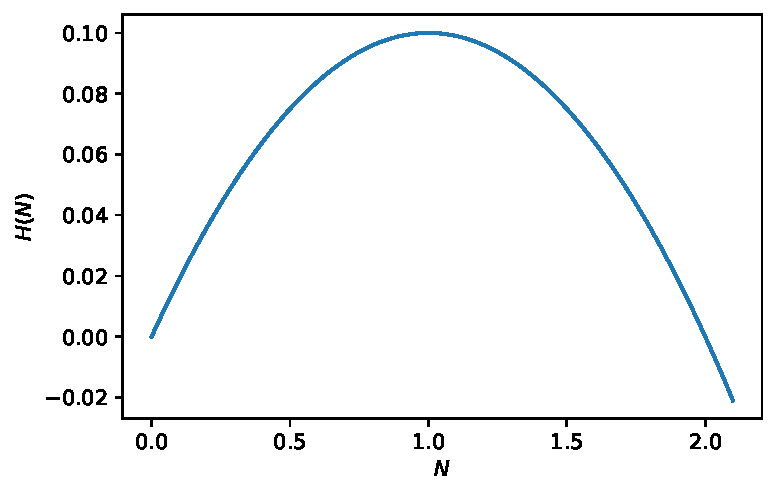
\includegraphics{SinglePopODEMOdels_files/figure-pdf/fig-dlogisticrhs-output-1.pdf}

}

\caption{\label{fig-dlogisticrhs}Right-hand side of the logistic ODE}

\end{figure}

\hypertarget{an-exact-solution}{%
\subsection{An exact solution}\label{an-exact-solution}}

Separation of variables yields \[
\int\frac{ dN}{N(1-\frac{N}{K})}=r\int dt.
\] Using partial fractions \[
\int\frac{ dN}{N} + \frac{1}{K}\int\frac{ dN}{1-\frac{N}{K}}=r\int dt.
\] Integration yields \[
\ln N - \ln\left(1-\frac{N}{K}\right)= \ln \frac{N }{1-\frac{N}{K}} =  rt+C.
\] Hence \[
N=\frac{De^{rt}}{1+\frac{D}{K}e^{rt}}
\] Given an initial condition \(N(0)=N_0\), we obtain \[
N(t)=\frac{N_0K e^{rt}}{K+N_0(e^{rt}-1)}
\]

\hypertarget{qualitative-analysis-of-the-exact-solution}{%
\subsubsection{Qualitative analysis of the exact
solution}\label{qualitative-analysis-of-the-exact-solution}}

As \(t\rightarrow \infty\), \(N\rightarrow K\). At \(t=0\), \(N=N_0\)
and that for small \(N_0\ll K\) the initial growth phase is exponential,
i.e.~ \[
N(t)\sim N_0 e^{rt} \\ \ \ \ \ N_0\ll K, t\ll \frac{1}{r}.
\]

Note that in almost all the models that we will consider the above
method is not an usually an option as the ODE is not explicitly
integrable.

\hypertarget{the-spruce-budworm-model}{%
\section{The spruce budworm model}\label{the-spruce-budworm-model}}

The spruce budworm is a destructive and widely distributed forest
defoliator in North America. Massive outbreaks occur periodically and
can destroy large quantities of valuable spruce and fir. To understand
the outbreak behaviour and develop and management strategies, a series
of mathematical models have been developed, beginning with Ludwig et al.
(1978). The goal of the models is to explain the qualitative pattern of
sudden outbreaks and then a sudden collapse.

\hypertarget{model-development-2}{%
\subsection{Model development}\label{model-development-2}}

Letting \(N(t)\) represent the population size at time \(t\), it is
assumed that budworm exhibits logistic growth and is subject to
predation at rate \(p(N)\). A governing ordinary differential equation
is given by \begin{equation}\protect\hypertarget{eq-sprucebudworm}{}{
\frac{dN }{dt}= r_B N\left(1-\frac{N}{K_B}\right)-p(N),
}\label{eq-sprucebudworm}\end{equation} where \[
p(N) =\frac{B N^2}{A^2 +N^2},
\] \(r_B\) is the linear growth rate, \(K_B\) is the carrying capacity,
\(B\) is the maximum rate of predation and \(A\) is a measure of budworm
population where predation switches on (specifically, \(A\) represents
the budworm density at which predation is half its maximum value).

It is informative to graph the predation term \[
p(N) =\frac{B N^2}{A^2 +N^2},
\] and annotate the parameters \(A\) and \(B\).

There is a root at \(N=0\). In the limit \(N\rightarrow \infty\),
\(p \rightarrow B\). Note that \(N=A\), \(p=A/2\). The derivative is \[
p'(N)=\frac{2BN}{A^2+N^2} - \frac{2BN^3}{(A^2+N^2)^2} =  \frac{2BA^2N}{(A^2+N^2)^2}
\] Thus there is a turning point at \(N=0\) and \(p'>0 \forall N>0\).

\hypertarget{nondimensionalisation-1}{%
\subsection{Nondimensionalisation}\label{nondimensionalisation-1}}

Introducing the (as yet unspecified) dimensional scalings \(\tilde{N}\)
and \(\tilde{T}\), the model is nondimensionalised as follows

\[
n=\frac{N}{\tilde{N}} \ \ \ \ \ \ \tau=\frac{t}{\tilde{T}}.
\]

Changing variables in Equation~\ref{eq-sprucebudworm} yields

\[
\frac{\tilde{N}}{\tilde{T}}\frac{d n }{d\tau}= r_B \tilde{N}n\left(1-\frac{\tilde{N}n}{K_B}\right)-\frac{B\tilde{N}^2n^2}{A^2+\tilde{N}^2 n^2}.
\]

After some tidying

\[
\frac{dn }{d\tau}= r_B\tilde{T} n\left(1-\frac{\tilde{N}n}{K_B}\right)-\frac{B\tilde{N} \tilde{T}}{A^2}\frac{n^2}{1+\frac{\tilde{N}^2}{A^2}n^2}.
\]

A natural scale for cell density in the model is given by the parameter
\(A\), as it determines the density of budworm at which predation is
half its maximal value. Hence we choose the scaling on the budworm
density \[
\tilde{N}=A.
\] Similarly, a natural time scale for the model is given by\\
\[
\tilde{T}=A/B.
\]

Substituting for \(\tilde{N}\) and \(\tilde{T}\) yields
\begin{equation}\protect\hypertarget{eq-budwormnondim}{}{
\frac{dn }{d\tau}= rn\left(1-\frac{n}{q}\right)-\frac{n^2}{1+n^2} = H(n),
}\label{eq-budwormnondim}\end{equation} where we define the
nondimensional parameters \[
r= \frac{r_B A}{B} \ \ \  \textrm{and} \ \ \  q=\frac{K_B}{A}.
\]

Note that Equation~\ref{eq-budwormnondim} has two nondimensional
parameters and all variables are dimensionless. See
Figure~\ref{fig-sprucebudworm-rhs} for a plot of right-hand side of
equation Equation~\ref{eq-budwormnondim}. What kind of behaviours do you
expect to see from the model?

\begin{figure}

{\centering 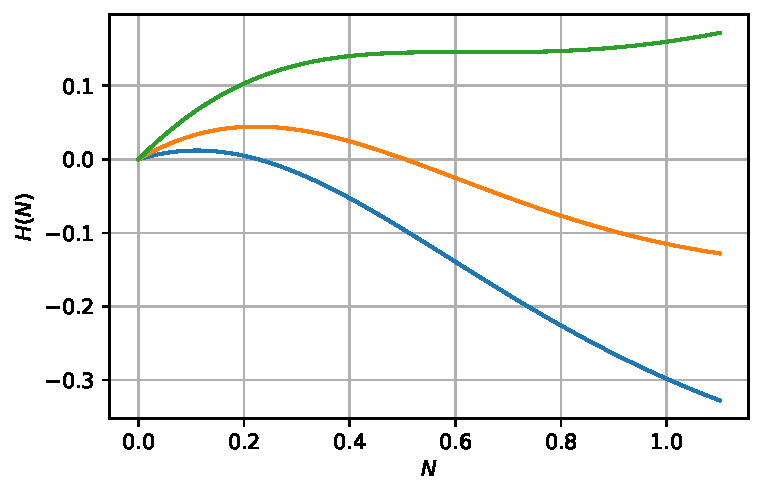
\includegraphics{SinglePopODEMOdels_files/figure-pdf/fig-sprucebudworm-rhs-output-1.pdf}

}

\caption{\label{fig-sprucebudworm-rhs}RHS of spr. budworm model}

\end{figure}

\hypertarget{numerical-solutions-1}{%
\subsection{Numerical solutions}\label{numerical-solutions-1}}

In Figure Figure~\ref{fig-sprucebudworm-numsol} we plot some numerical
solutions of Equation~\ref{eq-budwormnondim} at different values of the
parameter \(r\).

Numerical solutions of Equation~\ref{eq-budwormnondim} indicate that
there is a single stable steady state when \(r\) is both small and large
but for intermediate values of \(r\) there are two stable steady states.

Our goal is to analyse the model and understand why different parameter
values yield these strikingly different model behaviours.

\begin{figure}

{\centering 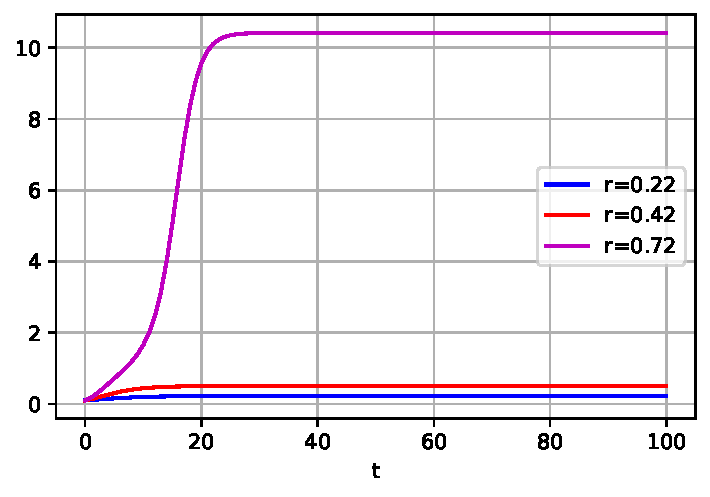
\includegraphics{SinglePopODEMOdels_files/figure-pdf/fig-sprucebudworm-numsol-output-1.pdf}

}

\caption{\label{fig-sprucebudworm-numsol}Numerical solution of spr.
budworm model}

\end{figure}

\hypertarget{steady-state-analysis}{%
\subsection{Steady state analysis}\label{steady-state-analysis}}

Letting \(n^*\) represent steady states of
Equation~\ref{eq-budwormnondim} yields \[
rn^*(1-\frac{n^*}{q})- \frac{n^*{^2}}{1+n^*{^2}}=0.
\] Hence either \[
n^*=0,
\] or \(n^*\) satisfies the cubic equation \[
r\left(1-\frac{n^*}{q}\right)- \frac{n^*}{1+n^*{^2}}=0.
\]

Explicit solutions to such a cubic can be immediately written down but
they are cumbersome to work with. We proceed using a
graphical/qualitative approach.

Define \begin{equation}\protect\hypertarget{eq-sprucebudwormfgn}{}{
f(n^*)=r\left(1-\frac{n^*}{q}\right) \ \ \textrm{and} \ \ g(n^*)=\frac{n^*}{1+n^*{^2}}.
}\label{eq-sprucebudwormfgn}\end{equation}

Roots occur for values of \(n^*\) that satisfy \(f=g\).

In Figure~\ref{fig-sprucebudworm-rhsfg} (a) we fix the parameter
\(q=10\) and consider model behaviour as a function of the parameter
\(r\). When \(r\gg1\) there is a nonzero steady-state corresponding to
\(n^*\gg 1\). When \(r\ll1\) there is a nonzero steady-state
corresponding to \(n^*\ll 1\). In the intermediate case there can be
three intersection points.

We can use the curve sketching techniques form Tutorial Sheet 1 to
sketch \(f\) and \(g\).

\(f\) is linear. There is a root at \(n^*=q\). The derivative is
\(-r/q\). \(f(0)\)=r. \(g\) has a unique root at \(n^*=0\). The
derivative is \[
g'=\frac{1-n{^*}^2}{(1+n^*)^2}.
\] There is a turning point at \(n^*=1\). Here \(g=1/2\). As
\(n^*\rightarrow \infty\), \(g\rightarrow 0\). \(f'(0)=1\).

\hypertarget{linear-stability-analysis-3}{%
\subsection{Linear stability
analysis}\label{linear-stability-analysis-3}}

The linear stability of the model is determined by the quantity \[
H'(n)=r(1-\frac{2n}{q})-\frac{2{n}}{1+{n}^2} +\frac{2{n}^3}{(1+{n}^2)^2}.
\]

Hence at the steady state \(n^*=0\) \[
H'(0)=r
\] and the steady state is linearly unstable.

Given the nonzero steady states have not been calculated explicitly, we
proceed using graphical analysis of stability. In
Figure~\ref{fig-sprucebudworm-rhsfg} (b) we plot the right-hand side of
Equation~\ref{eq-budwormnondim} against \(n\) and examine the cases of
large, small and intermediate \(r\) for a given value of \(q\).

When \(r\) is both large and small the nonzero steady state is stable
(the derivative at the roots is negative). In the case where three
biologically relevant roots exist, the intermediate root is unstable.

\begin{figure}

{\centering 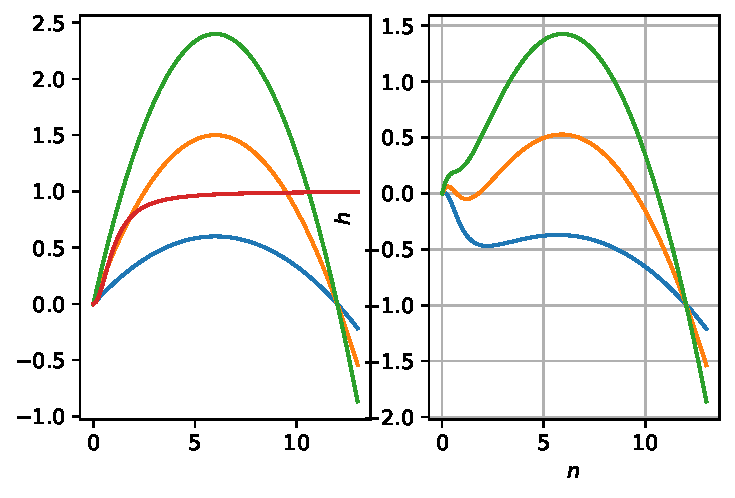
\includegraphics{SinglePopODEMOdels_files/figure-pdf/fig-sprucebudworm-rhsfg-output-1.pdf}

}

\caption{\label{fig-sprucebudworm-rhsfg}RHS of spr. budworm model}

\end{figure}

\hypertarget{bifurcation-analysis}{%
\subsection{Bifurcation analysis}\label{bifurcation-analysis}}

The goal is to identify boundaries of \(rq\) parameter space where the
stability changes occur and/or the number of steady states changes.

We can define points in \(rq\) parameter space where bifurcations arise
by seeking values of \(n^*\) that satisfy \[
f(n^*)= g(n^*) \ \ \ \  f'(n^*)= g'(n^*).
\]

The first of these equations yields
\begin{equation}\protect\hypertarget{eq-rqeqn1}{}{
  r(1-\frac{n^*}{q}) = \frac{n^*}{1+n{^*}^{2}},
}\label{eq-rqeqn1}\end{equation} and the latter yields
\begin{equation}\protect\hypertarget{eq-rqeqn2}{}{
 -\frac{r}{q}=\frac{1}{1+n{^*}^{2}}-\frac{2n{^*}^{2}}{(1+n{^*})^2} = \frac{1-n{^*}^{2}}{(1+n{^*}^{2})^2}.
}\label{eq-rqeqn2}\end{equation}

Hence \[
   \frac{r}{q}= \frac{n{^*}^{2}-1}{(1+n{^*}^{2})^2}.
\]

Substituting for \(r/q\) in the first equation yields \[
r-\frac{n{^*}^{2}-1}{(1+n{^*}^{2})^2}n^*=\frac{n^*}{1+n{^*}^{2}},
\] which can be written in the form \[
r=\frac{2n{^*}^{3}}{(1+n{^*}^{2})^2}.
\] Substituting for \(r\) in Equation~\ref{eq-rqeqn1} yields \[
\frac{2n{^*}^{3}}{(1+n{^*}^{2})^2}=\frac{2n{^*}^{3}}{(1+n{^*}^{2})^2}\frac{n^*}{q}+\frac{n^*}{1+n{^*}^2}
\] which, after some algebra, yields
\begin{equation}\protect\hypertarget{eq-sprucebudwormqpara}{}{
q=\frac{2n{^*}^3}{n{^*}^{2}-1}.
}\label{eq-sprucebudwormqpara}\end{equation} Hence a set of points that
define bifurcations where three steady states transform to a single
steady state are given in parametric form in \(qr\) parameter space by
\[
\left(\frac{2n{^*}^3}{n{^*}^{2}-1},\frac{2n{^*}^{3}}{(1+n{^*}^{2})^2}\right) \ \ \ \ \ \ \ n^*>1.
\]

\begin{verbatim}
/var/folders/m_/vc0kz_0x6ls5n4qnksq052jw0000gp/T/ipykernel_30906/3415590409.py:2: RuntimeWarning:

divide by zero encountered in divide
\end{verbatim}

\begin{figure}

{\centering 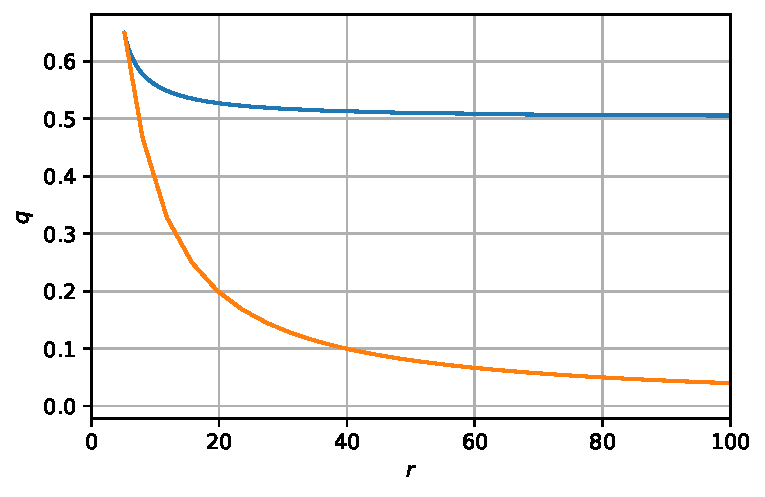
\includegraphics{SinglePopODEMOdels_files/figure-pdf/fig-sprucebudworm-rq-output-2.pdf}

}

\caption{\label{fig-sprucebudworm-rq}Bifurcations in the rq plane}

\end{figure}

By varying values of \(n^*\) in Figure~\ref{fig-sprucebudworm-rq} we
plot a region of instability. Note for example that
\(q\rightarrow \infty\) as \(n^*\rightarrow 1\) and as
\(n^*\rightarrow \infty\). Note also that in these limits \(r\) must
take the value 1/2 and 0, respectively.

We can show that the cusp in Figure~\ref{fig-sprucebudworm-rq} is given
by \[
\left(q,r\right)=\left(3^{\frac{3}{2}},\left(\frac{\sqrt{3}}{2}\right)^3\right).
\]

Note that \(r\) is a decreasing function of \(q\) for \(1<n^*<\sqrt{3}\)
but that \(r\) is an increasing function of \(n^*\) for
\(\sqrt{3}<n^*<\infty\). This can be shown by finding the turning points
of \(r\) w.r.t \(n^*\), i.e. Given that \[
r=\frac{2n{^*}^{3}}{(1+n{^*}^{2})^2},
\] differentiation with respect to \(n^*\) yields \[
\frac{dr}{dn^*}=\frac{6{n^*}^2}{(1+n^*)^2} - \frac{8n{^*}^4}{(1+n^*)^3}.
\] The turning point satisfies \[
\frac{6{n^*}^2}{(1+n^*)^2} - \frac{8n{^*}^4}{(1+n^*)^3}=0
\] Solving for \(n^*\) yields \[
6(1+{n^*}^2) - 8n{^*}^2=0 
\] Hence \[
  n^*=\sqrt{3}.
\] Thus there is a turning point that minimises \(r\) at
\(n^*=\sqrt{3}\).

Substitution for this value of \(n^*\) yields \[
\left(q,r\right)=\left(3^{\frac{3}{2}},\left(\frac{\sqrt{3}}{2}\right)^3\right).
\] See Figure~\ref{fig-sprucebudworm-rq}.

\hypertarget{hysteresis}{%
\subsection{Hysteresis}\label{hysteresis}}

Finally, rearranging the steady-state equation \[
  r(1-\frac{n^*}{q}) = \frac{n^*}{1+n{^*}^{2}},
 \] we obtain
\begin{equation}\protect\hypertarget{eq-sprucebudwormrpara}{}{ 
   r = \frac{n^*}{(1+n{^*}^{2})(1-\frac{n^*}{q})}.
}\label{eq-sprucebudwormrpara}\end{equation}

Considering \(n^*<q\) we compute \(r\); plotting \(n^*\) against \(r\)
yields the bifurcation curve presented in
Figure~\ref{fig-sprucebudworm-bfc}.

\begin{figure}

{\centering 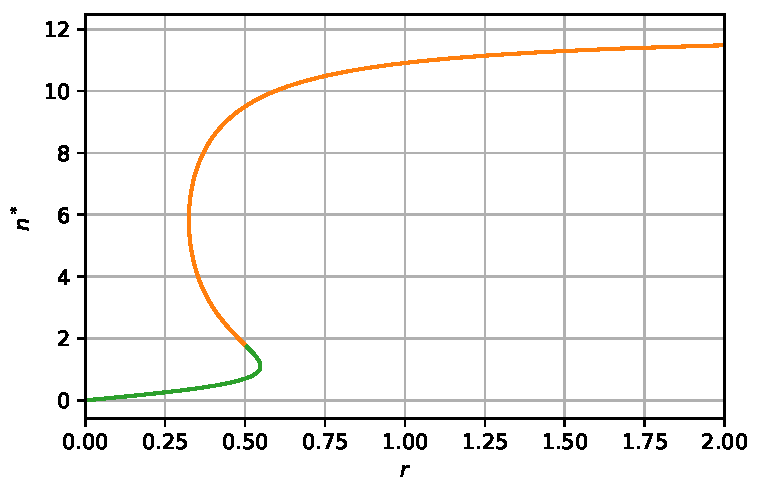
\includegraphics{SinglePopODEMOdels_files/figure-pdf/fig-sprucebudworm-bfc-output-1.pdf}

}

\caption{\label{fig-sprucebudworm-bfc}Bifurcations in the rq plane}

\end{figure}

A system exhibiting hysteresis shows a response to an increases in a
control parameter that is not exactly reversed when the parameter is
decreased. We can show that the spruce budworm model exhibits hysteresis
by considering the argument below.

Suppose \(r\) is initially small (\(r<r_1\)). There is only one
steady-state and any initial condition will converge towards it.

Suppose we increase the value of the parameter \(r\). There will be a
critical value of \(r\) (\(r=r_1\))where a second stable steady-state
arises and the model enters the bistable regime, where there are two
possible stable steady-states. Given the system system was originally in
the first stable steady state, it will remain there.

Suppose we continue to increase \(r\). Eventually we reach critical
value of \(r\) (\(r=r_2\)) where the first stable steady state is lost
and there is again only one stable steady-state.

Suppose we now decrease the parameter \(r\) below the threshold
\(r=r_2\). The system again enters the bistable regime but as the second
solution is stable, it remains the solution.

Suppose we continue to decrease \(r\) until eventually \(r<r_1\). We
return to the case where the system has only a single stable steady
state.

\hypertarget{harvesting}{%
\section{Harvesting}\label{harvesting}}

By introducing terms that represent harvesting, population models can be
used to investigate management strategies for resource management. The
modelling problem is to maximise the sustained yield.

Consider a model for logistic growth supplemented with a harvesting term
\[
\frac{dN}{dt}=rN\left(1-\frac{N}{K}\right) -EN.
\] The term \(EN\) is the harvesting yield per unit time and the
constant \(E\) represents the harvesting effort.

Steady states satisfy \[
rN^*\left(1-\frac{N^*}{K}\right) -EN^*=0
\] Thus either \(N^*=0\) or \[
\left(1-\frac{N^*}{K}\right) -E=0
\] Hence \[
N^*=K(1-\frac{E}{r}).
\] Note that this is positive only if \[
E<r.
\] Thus if the harvesting rate exceeds the linear growth rate the only
steady state corresponds to extinction.

The yield is \[
Y(E)=EN^*=EK(1-\frac{E}{r})
\]

To maximise the yields we differentiate with respect to \(E\). \[
\frac{dY}{dE} = K - 2\frac{EK}{r}.
\] Thus the maximum yield is identified by setting \[
\frac{dY}{dE} = K - 2\frac{EK}{r}=0.
\] THe maximum occurs at harvesting rate \[
E_c=\frac{r}{2}.
\] The maximum yield is \[
E^*=\frac{rK}{4}.
\]

We identify the time scale over which stocks return to steady state by
linearising about the steady state \(N^*=K(1-E/r)\), hence \[
\frac{d \hat{N}}{dt} = (E-r)\hat{N}.
\] Hence the recovery time scale is \[
T_R(E)=O(\frac{1}{r-E}).
\] As the harvesting rate approaches the linear growth rate \(r\), not
only does the steady state population tend to zero but the timescale for
stocks to recover tends to infinity. \}

\hypertarget{delay-differential-equation-models}{%
\section{Delay differential equation
models}\label{delay-differential-equation-models}}

Consider a model of the form \[
\frac{dN}{dt}=H(N(t),N(t-T)),
\] such that the right-hand side now depends on the value \(N\) not just
at time \(t\) but also at some delay time \(t-T\). We now need to
prescribe initial conditions of the form \[
N(t)=f(t), \quad -T<t\leq0.
\]

Consider a simple case of a linear model \[
\frac{dN}{dt}=-N(t-T).
\] A steady state, \(N^*\), is defined such that \(N(t)=N(t-T)=N^*\).
Hence \[
0=-kN^*.
\] The only steady state is \(N^*=0\).

To compute the linear stability we consider solution of the linearised
equation of the form \[
N(t)=e^{\lambda t}.
\] Hence \[
N(t-T)=e^{\lambda (t-T)}.
\]

Substitution yields \[
\lambda  e^{\lambda t} = - e^{\lambda (t-T)}.
\] Hence the eigenvalue, \(\lambda\), satisfies a transcendental
equation \[
\lambda=-e^{\lambda -T}.
\] This equation has no solutions for \(\lambda \in \Re\).

Consider solutions \(\lambda \in \mathbb{C}\). Let
\(\lambda=\mu+i\omega\). Substitution yields \[
\mu+i\omega = -e^{-\mu T}(\cos(\omega T)-i \sin(\omega T)).
\] Hence \[
\begin{aligned}
\mu=-\cos(\omega T)e^{-\mu T} \\
\omega = \sin(\omega T)e^{-\mu T}.
\end{aligned}
\] For linear stability we require that \(\mu <0\). This implies that \[
-\frac{\pi}{2}<\omega T < \frac{\pi}{2}.
\]

Consider \[
\frac{e^{\mu T}}{T}=\frac{\omega e^{\mu T}}{\omega T} = \frac{\sin(\omega T)}{\omega T}
\]

Noting that \[
\frac{\sin z}{z} > \frac{1}{\frac{\pi}{2}}
\] yields \[
 \frac{\sin(\omega T)}{\omega T}>\frac{2}{\pi}.
\] Hence \[
\frac{e^{\mu T}}{T} >\frac{2}{\pi}.
\] Rearranging \[
T<\frac{\pi}{2}e^{\mu T}.
\] For linear stability \(\mu<0\). Hence a necessary condition for
linear stability is that \[
T<\frac{\pi}{2}
\]

\hypertarget{references-1}{%
\section{References}\label{references-1}}

\hypertarget{multi-species-population-dynamics-1}{%
\chapter{Multi species population
dynamics}\label{multi-species-population-dynamics-1}}

In this chapter we consider models of interacitng populations.

Let \(u=u(t)\) and \(v=v(t)\) represent populations of two different
species at continuous time \(t\). Suppose that \(u(t)\) and \(v(t)\)
satisfy the ordinary differential equations
\begin{equation}\protect\hypertarget{eq-twovariablfegen}{}{
\begin{aligned}
\frac{du}{dt}&=f(u,v),  \nonumber \\
\frac{dv}{dt}&=g(u,v).
\end{aligned}
}\label{eq-twovariablfegen}\end{equation}

In this section we will consider particular forms for \(f\) and \(g\)
that represent different types of inter species interaction. Before
considering particular examples, we develop some general techniques for
analysing equations of the form Equation~\ref{eq-twovariablfegen}.

\hypertarget{general-tools}{%
\section{General tools}\label{general-tools}}

\hypertarget{steady-states}{%
\subsection{Steady states}\label{steady-states}}

\((u^*,v^*)\) is defined to be a steady state of
Equation~\ref{eq-twovariablfegen} if

\[
f(u^*,v^*)=g(u^*,v^*)=0.
\]

Hence, by definition, the time derivatives of \(u(t)\) and \(v(t)\) are
both zero at \((u^*,v^*)\). As was the case for single species models,
steady states are obtained by solving algebraic equations.

\begin{tcolorbox}[enhanced jigsaw, bottomtitle=1mm, rightrule=.15mm, colback=white, leftrule=.75mm, title=\textcolor{quarto-callout-note-color}{\faInfo}\hspace{0.5em}{Note}, bottomrule=.15mm, coltitle=black, toptitle=1mm, breakable, colframe=quarto-callout-note-color-frame, titlerule=0mm, toprule=.15mm, opacitybacktitle=0.6, arc=.35mm, colbacktitle=quarto-callout-note-color!10!white, left=2mm, opacityback=0]

Compute the steady states of the system of ODEs \[
\begin{aligned}
\frac{du}{dt}&=1-u,  \nonumber \\
\frac{dv}{dt}&=1-uv-v.
\end{aligned}
\]

\end{tcolorbox}

\begin{tcolorbox}[enhanced jigsaw, bottomtitle=1mm, rightrule=.15mm, colback=white, leftrule=.75mm, title=\textcolor{quarto-callout-tip-color}{\faLightbulb}\hspace{0.5em}{Tip}, bottomrule=.15mm, coltitle=black, toptitle=1mm, breakable, colframe=quarto-callout-tip-color-frame, titlerule=0mm, toprule=.15mm, opacitybacktitle=0.6, arc=.35mm, colbacktitle=quarto-callout-tip-color!10!white, left=2mm, opacityback=0]

Suppose \((u^*,v^*)\) is a steady state. Hence \[
 0=1-u^*
 \] and \[
 0=1-u^*v^*-v^*
 \] The steady state is \((1,1/2)\).

\end{tcolorbox}

\hypertarget{linear-stability-analysis-4}{%
\subsection{Linear stability
analysis}\label{linear-stability-analysis-4}}

Suppose that \((u^*,v^*)\) is a steady state of equations
Equation~\ref{eq-twovariablfegen}.

We consider a change of dependent variables such that

\[
u(t)=u^*+ \hat{u}(t)  \  \  \textrm{and} \ \ v(t)=v^*+\hat{v}(t),
\]

where \(\hat{u}(t)\) and \(\hat{v}(t)\) are perturbations about the
steady state.

Rewriting equation Equation~\ref{eq-twovariablfegen} in the transformed
variables yields

\begin{equation}\protect\hypertarget{eq-twovariablfegentrans}{}{
\begin{aligned}
\frac{d\hat{u}}{dt}&=f(u^*+\hat{u},v^*+\hat{v}),  \nonumber \\
\frac{d\hat{v}}{dt}&=g(u^*+\hat{u},v^*+\hat{v}).
\end{aligned}
}\label{eq-twovariablfegentrans}\end{equation}

Making Taylor expansions about \((u^*,v^*)\) yields the linearised
equations

\begin{equation}\protect\hypertarget{eq-twovariablfegenlin}{}{
\begin{aligned}
\frac{d\hat{u}}{dt}=\frac{\partial f}{\partial u}_{|(u^*,v^*)} \hat{u} +  \frac{\partial f}{\partial v}_{|(u^*,v^*)}  \hat{v} + h.o.t, \nonumber\\
\frac{d\hat{v}}{dt}=\frac{\partial g}{\partial u}_{|(u^*,v^*)}  \hat{u} +  \frac{\partial g}{\partial v}_{|(u^*,v^*)}  \hat{v} + h.o.t. \nonumber
\end{aligned}
}\label{eq-twovariablfegenlin}\end{equation}

Upon making the assumption that the perturbations about the steady state
are small, the leading order terms are linear and higher order terms are
neglected. Defining

\[
\mathbf{w}=\left
(\begin{array}{r}
\hat{u} \\ 
\hat{v} 
\end{array}\right),
\]

yields the system of linear ODEs given by

\begin{equation}\protect\hypertarget{eq-linearsystem2d}{}{
\frac{d \mathbf{w}}{dt}= A \mathbf{w},
}\label{eq-linearsystem2d}\end{equation}

where the matrix \(A\), known as the Jacobian matrix, takes the form

\[
A=\left(\begin{array}{rr}
\frac{\partial f}{\partial u}&\frac{\partial f}{\partial v} \\ \frac{\partial g}{\partial u}&\frac{\partial g}{\partial v} \end{array}\right)_{(u^*,v^*)}. \qquad
\]

The linear system arrived upon in Equation~\ref{eq-linearsystem2d} was
encountered previously in Differential Equations (MA31002). We summarise
the important results here. Seeking a solution of
Equation~\ref{eq-linearsystem2d} of the form

\[
\mathbf{w}=\mathbf{v}e^{\lambda t}
\]

one obtains the characteristic equation

\[
\lambda^2 -\lambda \mathrm{tr}(A)+\det(A)=0,
\] which has solutions

\[
\lambda = \frac{\mathrm{tr}{A}\pm \sqrt{\mathrm{tr}{A}^2-4\det{A}}}{2}.
\]

Whilst a complete classification of the linear stability of a steady
state can be obtained by explicitly calculating the eigenvalues, in many
cases it is sufficient to deduce whether or not a steady state is stable
or unstable. This can be achieved by calculating the determinant and
trace of the Jacobian matrix (\(\det(A)\) and \(\mathrm{tr}(A)\),
respectively) and referring to Figure~\ref{fig-tdplane}.

\begin{figure}

{\centering 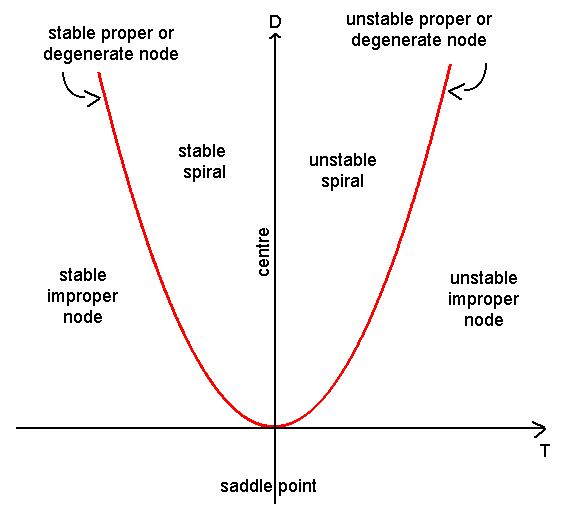
\includegraphics{TDPlane.png}

}

\caption{\label{fig-tdplane}Stability in the trace detemrinant plane.}

\end{figure}

The different cases can be categorised as follows:

\begin{itemize}
\item
  \(\det(A)<0\) There is one positive and one negative real eigenvalue.
  Hence the steady state is a saddle which is unstable.
\item
  \(\det(A)>0\) The steady state can be either stable or unstable,
  depending on \(\mathrm{tr}(A)\) (and the real part of the
  eigenvalues).

  \begin{itemize}
  \tightlist
  \item
    If \(\mathrm{tr}(A)>0\), the steady state is unstable.

    \begin{itemize}
    \tightlist
    \item
      If \(\mathrm{tr}(A)^2>4 \det(A)\), it is an unstable node.
    \item
      If \(\mathrm{tr}(A)^2<4 \det(A)\) it is an unstable spiral.
    \end{itemize}
  \item
    If \(\mathrm{tr}(A)<0\), the steady state is stable.

    \begin{itemize}
    \tightlist
    \item
      If \(\mathrm{tr}(A)^2>4 \det(A)\), it is an stable node.
    \item
      If \(\mathrm{tr}(A)^2<4 \det(A)\), it is an stable spiral.
    \end{itemize}
  \end{itemize}
\end{itemize}

These different cases can be distinguished in the trace-determinant
plane plotted in Figure~\ref{fig-tdplane}.

Note that it can be shown rigorously that the linear stability of the
nonlinear system is equivalent to that of the linearised system in all
cases except when the steady state is a centre. In this case, nonlinear
stability analysis is required to determine the stability of the
nonlinear system.

\begin{tcolorbox}[enhanced jigsaw, bottomtitle=1mm, rightrule=.15mm, colback=white, leftrule=.75mm, title=\textcolor{quarto-callout-note-color}{\faInfo}\hspace{0.5em}{Note}, bottomrule=.15mm, coltitle=black, toptitle=1mm, breakable, colframe=quarto-callout-note-color-frame, titlerule=0mm, toprule=.15mm, opacitybacktitle=0.6, arc=.35mm, colbacktitle=quarto-callout-note-color!10!white, left=2mm, opacityback=0]

Deduce, by considering the form for the eigenvalues that, for example,
the conditions \(\det(A)>0\), \(\mathrm{tr}(A)>0\) with
\(\mathrm{tr}(A)^2<4 \det(A)\) imply that the steady state is an
unstable spiral.

\end{tcolorbox}

\begin{tcolorbox}[enhanced jigsaw, bottomtitle=1mm, rightrule=.15mm, colback=white, leftrule=.75mm, title=\textcolor{quarto-callout-tip-color}{\faLightbulb}\hspace{0.5em}{Tip}, bottomrule=.15mm, coltitle=black, toptitle=1mm, breakable, colframe=quarto-callout-tip-color-frame, titlerule=0mm, toprule=.15mm, opacitybacktitle=0.6, arc=.35mm, colbacktitle=quarto-callout-tip-color!10!white, left=2mm, opacityback=0]

The eigenvalues are given by \[
\lambda = \frac{\mathrm{tr}{A}\pm \sqrt{\mathrm{tr}{A}^2-4\det{A}}}{2}
\] The condition\(\det(A)>0\) excludes the case that the eigenvalues are
real but have opposite signs (i.e.~it cannot be a saddle point).

The condition \(\mathrm{tr}(A)>0\) implies that the real part of both
eigenvalues are positive (i.e.~the steady state is unstable).

The condition \(\mathrm{tr}(A)^2<4 \det(A)\) implies that the eigenvalue
are complex. Hence \[
\lambda_{\pm}=\mu\pm i\omega \ \ \ 
\] and the solution of the system can be written \[
e^{\lambda t} = e^{(\mu+i\omega) t} = e^{\mu t}e^{i\omega t}. 
\] Thus the magnitude of perturbation grows but it oscillates about the
steady state. Hence the steady state is an unstable spiral.

\end{tcolorbox}

\begin{tcolorbox}[enhanced jigsaw, bottomtitle=1mm, rightrule=.15mm, colback=white, leftrule=.75mm, title=\textcolor{quarto-callout-note-color}{\faInfo}\hspace{0.5em}{Note}, bottomrule=.15mm, coltitle=black, toptitle=1mm, breakable, colframe=quarto-callout-note-color-frame, titlerule=0mm, toprule=.15mm, opacitybacktitle=0.6, arc=.35mm, colbacktitle=quarto-callout-note-color!10!white, left=2mm, opacityback=0]

Compute the Jacobian matrix for the system of ODEs \[
\begin{aligned}
\frac{du}{dt}&=1-u,  \nonumber \\
\frac{dv}{dt}&=1-uv-v.
\end{aligned}
\] Evaluate the Jacobian matrix at the steady state and hence determine
its linear stability.

\end{tcolorbox}

\begin{tcolorbox}[enhanced jigsaw, bottomtitle=1mm, rightrule=.15mm, colback=white, leftrule=.75mm, title=\textcolor{quarto-callout-tip-color}{\faLightbulb}\hspace{0.5em}{Tip}, bottomrule=.15mm, coltitle=black, toptitle=1mm, breakable, colframe=quarto-callout-tip-color-frame, titlerule=0mm, toprule=.15mm, opacitybacktitle=0.6, arc=.35mm, colbacktitle=quarto-callout-tip-color!10!white, left=2mm, opacityback=0]

The Jacobian is given by \[
A=\left(\begin{array}{rr} -1&0 \\ -v &-u-1 \end{array}\right).
\] At (1,1/2) \[
A=\left(\begin{array}{rr} -1&0 \\ -\frac{1}{2} &-2 \end{array}\right).
\] In this case \[
 tr(A)=-3
 \] and \[
 \det(A)=2
 \] Hence the steady state is stable. As \[
 tr(A)^2-4\det(A)=9-8=1,
 \] it is a stable node.

\end{tcolorbox}

\hypertarget{nullclines}{%
\subsection{Nullclines}\label{nullclines}}

Nullclines of the equations Equation~\ref{eq-twovariablfegen} are given
by the curves \[
f(u,v)=0
\] and \[
 g(u,v)=0,
\] respectively. Note that steady states arise at the intersection of
nullclines.

Using the \(u\) nullclines we identify domains of the phase plane where
\(du/dt >0\) and \(du/dt <0\).

Similarly, using the \(v\) nullcline we identify domains of the phase
plane where \(dv/dt >0\) and \(dv/dt <0\).

The nullclines can be used to help identify confined sets and hence
apply the Poincaire-Bendixson theorem.

\begin{tcolorbox}[enhanced jigsaw, bottomtitle=1mm, rightrule=.15mm, colback=white, leftrule=.75mm, title=\textcolor{quarto-callout-note-color}{\faInfo}\hspace{0.5em}{Note}, bottomrule=.15mm, coltitle=black, toptitle=1mm, breakable, colframe=quarto-callout-note-color-frame, titlerule=0mm, toprule=.15mm, opacitybacktitle=0.6, arc=.35mm, colbacktitle=quarto-callout-note-color!10!white, left=2mm, opacityback=0]

Sketch the nullclines of the system of ODEs \[
\begin{aligned}
\frac{du}{dt}&=1-u,  \nonumber \\
\frac{dv}{dt}&=1-uv-v.
\end{aligned}
\]

\end{tcolorbox}

\begin{tcolorbox}[enhanced jigsaw, bottomtitle=1mm, rightrule=.15mm, colback=white, leftrule=.75mm, title=\textcolor{quarto-callout-tip-color}{\faLightbulb}\hspace{0.5em}{Tip}, bottomrule=.15mm, coltitle=black, toptitle=1mm, breakable, colframe=quarto-callout-tip-color-frame, titlerule=0mm, toprule=.15mm, opacitybacktitle=0.6, arc=.35mm, colbacktitle=quarto-callout-tip-color!10!white, left=2mm, opacityback=0]

The \(u\) nullcline is \(u=1\). The \(v\) nullcline is \(v=1/(1+u)\).

\end{tcolorbox}

\hypertarget{poincaire-bendixson-theorem}{%
\subsection{Poincaire-Bendixson
theorem}\label{poincaire-bendixson-theorem}}

Suppose that the system of equations
\begin{equation}\protect\hypertarget{eq-xygenphaseplane}{}{
\frac{du}{dt}=f(u,v), \ \ \ \ \frac{dv}{dt}=g(u,v)
}\label{eq-xygenphaseplane}\end{equation} possesses a confined set
(i.e.~a bounded domain in the phase plane upon which the derivative
field points into the domain) that contains an unstable node or spiral.
Any trajectory cannot leave the confined set, nor can it tend to the
unstable steady state. The Poincaire-Bendixson theorem states that as
\(t\rightarrow \infty\), the trajectory will tend towards a limit cycle.

\hypertarget{dulac-criterion}{%
\subsection{Dulac criterion}\label{dulac-criterion}}

Suppose \(D\) is a simply connected region in the plane and that there
exists a function \(B(x,y)\), continuously differentiable on \(D\), such
that the expression \[
\frac{\partial }{\partial u} (Bf) + \frac{\partial }{\partial v} (Bg)
\] is not identically zero and does not change sign in D. Then there are
no closed orbits in \(D\).

\hypertarget{the-lotka-voltera-model}{%
\section{The Lotka-Voltera model}\label{the-lotka-voltera-model}}

Suppose that \(N(t)\) and \(P(t)\) represent the prey and predator
population densities at time \(t\), respectively. Consider a model of
the form \[
   \begin{aligned}
   \frac{dN }{dt} &= aN -bNP, \nonumber \\
      \frac{dP }{dt} &= cNP -dP, 
\end{aligned}
\] where \(a\), \(b\), \(c\) and \(d\) are positive constants.

\hypertarget{nondimensionalisation-2}{%
\subsection{Nondimensionalisation}\label{nondimensionalisation-2}}

Nondimensionalising with \[
n=\frac{N}{\tilde{N}}, \ \ \ \ p=\frac{P}{\tilde{P}}  \ \ \textrm{and} \ \ \tau= \frac{t}{\tilde{T}},
\]

yields, after changing variables, \[  
 \begin{aligned}
   \frac{dn }{d\tau} &= \tilde{T}an -b\tilde{T} \tilde{P}np,  \nonumber \\
      \frac{dp }{d\tau} &= c\tilde{N} \tilde{T}np -d\tilde{T}p. 
\end{aligned}
\] Choosing the dimensional scalings

\[
\tilde{T}=1/a, \ \ \ \tilde{P}=a/b  \ \ \ \textrm{and} \ \ \ \tilde{N}=d/c,
\]

yields

\begin{equation}\protect\hypertarget{eq-lotkavolterranondim}{}{
\begin{aligned}
 \frac{dn }{d\tau} &= n(1-p) = f(n,p), \nonumber \\
 \frac{dp }{d\tau} &=\alpha p(n-1)  = g(n,p),
\end{aligned} 
}\label{eq-lotkavolterranondim}\end{equation}

where \(\alpha=d/a\). Note that all variables and parameter are without
dimensions.

\hypertarget{numerical-solutions-2}{%
\subsection{Numerical solutions}\label{numerical-solutions-2}}

\begin{figure}

{\centering 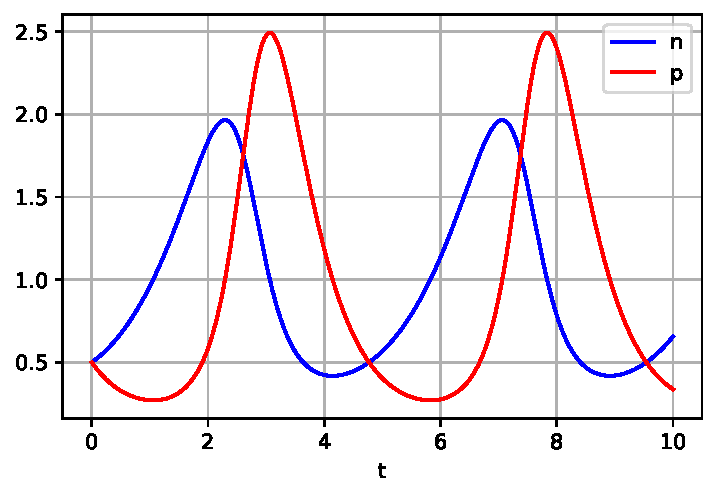
\includegraphics{ContinuousTimeTwoSepcies_files/figure-pdf/fig-lv-numsol-output-1.pdf}

}

\caption{\label{fig-lv-numsol}Numerical solution of Lotka-Volterra
model}

\end{figure}

\hypertarget{steady-states-1}{%
\subsection{Steady states}\label{steady-states-1}}

The steady-states of equation Equation~\ref{eq-lotkavolterranondim} are
identified by seeking solutions of

\[
f(n^*,p^*)=g(n^*,p^*)=0.
\]

Hence

\[
n^*(1-p^*)= 0 \ \ \ \ \ \alpha p^*(n^*-1).
\]

The first of these equations has solutions either

\[
n^*=0 \ \ \  \textrm{or} \ \ \  p^* =1.
\]

Substituting for \(n^*=0\) in the second equation yields \(p^*=0\).
Hence one steady state is \((0,0)\). Substituting for \(p^*=1\) in the
second equation yields \(n^*=1\). Hence a second steady state is (1,1).

\hypertarget{linear-stability-3}{%
\subsection{Linear stability}\label{linear-stability-3}}

The linear stability of the steady states is described by the Jacobian
matrix \[
A=\left(\begin{array}{rr}
\frac{\partial f}{\partial n}&\frac{\partial f}{\partial p} \\ \frac{\partial g}{\partial n}&\frac{\partial g}{\partial p} \end{array}\right)_{(n^*,p^*)} = \left(\begin{array}{rr}
1-p&-n \\ \alpha p &\alpha (n-1) \end{array}\right)_{(n^*,p^*)} 
\]

Evaluating at (0,0) yields

\[
A=\left(\begin{array}{rr} 1&0 \\ 0 &-\alpha \end{array}\right),
\]

Hence the eigenvalues of \(A\) are \(1\) and \(-\alpha\). As
\(\alpha>0\) the origin is a saddle. The eigenvectors are \([1, 0]\) and
\${[}0,1{]}. \$

At (1,1) \[
A=\left(\begin{array}{rr} 0&-1 \\ \alpha &0 \end{array}\right),
\]

and the eigenvalues are \(\pm i\sqrt{\alpha}\). Therefore the steady
state at (1,1) is a centre.

\hypertarget{solutions-in-the-phase-plane}{%
\subsection{Solutions in the phase
plane}\label{solutions-in-the-phase-plane}}

See Figure~\ref{fig-lv-numsol-phplane} for solution trajectories plotted
in the phase plane using different initial conditions. Note the expected
saddle like behaviour when trajectories that are close to the origin.
Furthermore, note that the different initial conditions result in
distinct closed loops and that the inner-most loop, i.e.~that closest to
the steady-state (1,1), behaves like a centre, as expected given the
linear stability analysis. However, far from the steady-state the
solution trajectory deviates from the linearised model.

\begin{figure}

{\centering 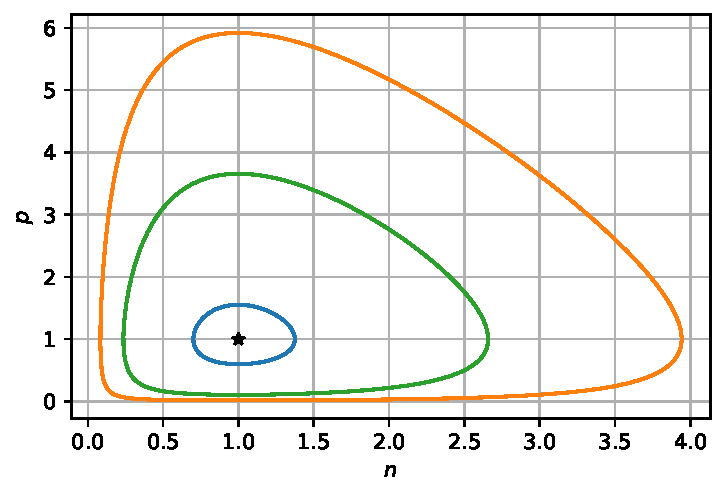
\includegraphics{ContinuousTimeTwoSepcies_files/figure-pdf/fig-lv-numsol-phplane-output-1.pdf}

}

\caption{\label{fig-lv-numsol-phplane}Numerical solution of
Lotka-Volterra model}

\end{figure}

\hypertarget{direct-integration}{%
\subsection{Direct integration}\label{direct-integration}}

The Lotka-Volterra equations are a special case as they are integrable.
Trajectories in the phase plane satisfy the differential equation

\[
\frac{dp }{d n} = \frac{\alpha p (n-1)}{n(1-p)},
\]

Using separation of variables

\[
\int \frac{1-p}{p} dp  = \alpha  \int \frac{n-1}{n} dn.  
\]

Integration yields

\[
\ln p - p =  \alpha (n-\ln n) + H,
\]

where \(H\) is a conserved quantity that this is determined by the
initial conditions. As the equations take conservative form, the
Lotka-Voltera model is said to be structurally unstable, as a small
perturbation to the solution at a given point in the oscillatory cycle
can result in large changes elsewhere in the cycle. For example, suppose
the outermost limit cycle in Figure~\ref{fig-lv-numsol-phplane} is
perturbed by a small amount at the point (1,0.1) onto its nearest limit
cycle. Later in the cycle these two trajectories deviate by a large
amount.

\hypertarget{competition}{%
\section{Competition}\label{competition}}

In models of competition, two or more species compete for the same
resource or in some way inhibit each other's growth. Letting \(N_1(t)\)
and \(N_2(t)\) represent the population density of two species, we
consider the ODEs \[
\begin{aligned}
\frac{d N_1}{dt} &= r_1N_1\left(1-\frac{N_1}{K_1}-b_{12}\frac{N_2}{K_1}\right), \nonumber \\
\frac{d N_2}{dt} &= r_2N_2\left(1-\frac{N_2}{K_2}-b_{21}\frac{N_1}{K_2}\right), 
\end{aligned}
\] where \(r_1\), \(r_2\), \(K_1\) and \(K_2\) are positive constants.
As before, the \(r's\) are linear growth rates and the \(K\)'s are
carrying capacities. The parameters \(b_{12}\) and \(b_{21}\) measure
the competitive effect of \(N_2\) on \(N_1\) and \(N_1\) on \(N_2\),
respectively.

\hypertarget{nondimensionalisation-3}{%
\subsection{Nondimensionalisation}\label{nondimensionalisation-3}}

After nondimensionalising using the change of variables

\[
n_1=\frac{N_1}{K_1} \ \ n_2=\frac{N_2}{K_2} \ \ \tau=\frac{t}{\frac{1}{r_1}},
\]

we obtain the equations

\begin{equation}\protect\hypertarget{eq-competitionnondim}{}{
\begin{aligned}
\frac{d n_1}{d\tau} &= n_1\left(1- n_1-a_{12}n_2\right) = f(n_1,n_2), \nonumber \\
\frac{d n_2}{d\tau} &= \rho n_2\left(1-n_2-a_{21}n_1\right) =g(n_1,n_2),
\end{aligned}
}\label{eq-competitionnondim}\end{equation}

where

\[
\rho=\frac{r_2}{r_1}, \ \ \ a_{12}=b_{12}\frac{K_2}{K_1}, \ \ \  a_{21}=b_{21}\frac{K_1}{K_2}. 
\]

\hypertarget{steady-states-2}{%
\subsection{Steady states}\label{steady-states-2}}

The steady states of Equation~\ref{eq-competitionnondim} are identified
in the usual manner, i.e.~by seeking \(({n_1}^*,{n_2}^*)\) such that

\[
f({n_1}^*,{n_2}^*)=g({n_1}^*,{n_2}^*)=0.
\]

The steady state equations are \[
 {n_1}^*\left(1- {n_1}^*-a_{12}{n_2}^*\right)=0 \ \ \ \ {n_2}^*\left(1-{n_2}^*-a_{21}{n_1}^*\right)=0.
\] The first equation has solution \[
n_1^*=0
\] or \[
\left(1- {n_1}^*-a_{12}{n_2}^*\right) \implies n_2=\frac{1}{a_{12}}(1-n_1^*).
\] Consider \(n_1^*=0\). Substitution in the second equation yields \[
 {n_2}^*\left(1-{n_2}^*\right)=0.
 \] Hence either \(n_2^*=0\) or \(n_2^*=1\). Hence two steady states are
\((0,0)\) and \((0,1).\) \textbackslash{} Now consider
\(n_2^*=\frac{1}{a_{12}}(1-n_1^*)\) with \(n_1^*\neq0\).
\textbackslash{} Substitution in the second steady state equation yields
\[
\frac{1}{a_{12}}(1-n_1^*) \left(1- \frac{1}{a_{12}}(1-n_1^*) -a_{21}{n_1}^*\right)
 \] Hence either \(n_1^*=1\) or \[
 \left(1- \frac{1}{a_{12}}(1-n_1^*) -a_{21}{n_1}^*\right)=0 \implies n_1^*=\frac{1-a_{12}}{1-a_{12}a_{21}}.
 \] In the case where \(n_1^*=1\), we find that \(n_2^*=0\). Hence the
steady state is (1,0).

In the case where \[
n_1^*=\frac{1-a_{12}}{1-a_{12}a_{21}}
\] we find that \[
n_2^*=\frac{1-a_{21}}{1-a_{12}a_{21}}
\] Hence the steady state is \[
\left(\frac{1-a_{12}}{1-a_{12}a_{21}},\frac{1-a_{21}}{1-a_{12}a_{21}}\right).
\]

\hypertarget{nullclines-1}{%
\subsection{Nullclines}\label{nullclines-1}}

The nullclines for Equation~\ref{eq-competitionnondim} are straight
lines given by

\[
 n_1=0 \ \ \ \ \ n_2=\frac{1-n_1}{a_{12}}, 
 \]

and

\[ 
 n_2=0 \ \  \ \  \ n_2= 1-a_{21}n_1.
 \]

Note that the steady states \((0,0)\), \((1,0)\) and \((0,1)\) are
always biologically relevant (i.e.~independently of the parameter values
for \(a_{12}\) and \(a_{21}\)).

However, the coexistence steady state is only biologically relevant if
the nullclines intersect in the positive quadrant and this occurs only
in certain regions of the model's parameter space.

In the cases where \(a_{12},a_{21}<1\) and \(a_{12},a_{21}>1\) there is
a coexistence steady state (i.e.~the nullclines intersect in the
positive quadrant).

However, if \(a_{21}<1\) and \(a_{12}>1\) or \(a_{12}<1\) and
\(a_{21}>1\) there is not a biologically relevant, coexistence steady
state (i.e.~the nullclines do not intersect in the positive quadrant).

Hence there are are four qualitatively different types of solution to
consider.

\hypertarget{linear-stability-4}{%
\subsection{Linear stability}\label{linear-stability-4}}

The linear stability of the different steady states is determined by
calculating the Jacobian matrix

\[
A=\left(\begin{array}{rr}
\frac{\partial f}{\partial n_1}&\frac{\partial f}{\partial n_2} \\ \frac{\partial g}{\partial n_1 }&\frac{\partial g}{\partial n_2} \end{array}\right)_{({n_1}^*,{n_2}^*)} = \left(\begin{array}{rr}
1-2n_1 -a_{12}n_2&-a_{12}n_1 \\ -\rho a_{21}n_2 &\rho(1-2n_2-a_{21}n_1)\end{array}\right)_{({n_1}^*,{n_2}^*)}. 
\]

At (0,0)

\[
A=\left(\begin{array}{rr}
1& 0 \\ 0 & \rho\end{array}\right). 
\]

Hence the eigenvalues of the Jacobian are \(1\) and \(\rho\). As
\(\rho>0\), the origin is therefore an unstable node (there are two real
positive eigenvalues).

At (1,0)

\[
A=\left(\begin{array}{rr}
-1& -a_{12} \\ 0 & \rho(1-a_{21})\end{array}\right). 
\]

The trace and determinant are given by

\[
\det{A}=\rho  (a_{21}-1)\ \ \ \textrm{and} \ \ \ \mathrm{tr}{A}=-1+\rho(1-a_{21}).
\]

Hence if \(a_{21}<1\), \(\det{A}<0\) and (1,0) is a saddle point and
thus unstable (see Figure~\ref{fig-tdplane}).

If \(a_{21}>1\), \(\det{A}>0\) and \(\mathrm{tr}{A}<0\). Hence (1,0) is
a stable node.

Hence the parameter \(a_{21}\), which describes how strongly Population
1 inhibits the growth rate of Population 2, determines whether or not
the steady state representing extinction of Population 2 but not
Population 1 is stable or not.

At (0,1)

\[
A=\left(\begin{array}{rr}
1-a_{12}& 0\\  -\rho a_{21} & -\rho \end{array}\right). 
\]

In this case if \(a_{12}<1\), \(\det{A}<0\) and (0,1) is a saddle point.
If \(a_{12}>1\), \(\det{A}>0\) and \(\mathrm{tr}{A}<0\) and (0,1) is a
stable node. Hence the parameter \(a_{12}\), which describes how
strongly Population 2 inhibits the growth rate of Population 1,
determines whether or not the steady state representing extinction of
Population 1 but not Population 2 is stable or not.

At the coexistence steady state, recall the steady state is

\[
\left(\frac{1-a_{12}}{1-a_{12}a_{21}},\frac{1-a_{21}}{1-a_{12}a_{21}}\right).
\] Note that this steady state is only biologically relevant in the
cases \(a_{21}<1, a_{12}<1\) or \(a_{21}>1, a_{12}>1\). Evaluating the
Jacobian yields \[
A=\frac{1}{1-a_{12}a_{21}}\left(\begin{array}{rr}
a_{12}-1  & -a_{12}(1-a_{12})\\ -\rho a_{21}(1-a_{21}) &\rho(a_{21}-1)\end{array}\right). 
\]

The determinant and trace of the Jacobian are given by

\[
\begin{aligned}
\det{A}&=\rho\left((a_{12}-1)(a_{21}-1)-a_{12}a_{21}(1-a_{12})(1-a_{21})\right)\frac{1}{(1-a_{12}a_{21})^2}, \nonumber \\
&= \rho\frac{(a_{12}-1)(a_{21}-1)}{(1-a_{12}a_{21})},
\end{aligned}
\]

and

\[
\mathrm{tr}{A}=\left(a_{12}-1+\rho(a_{21}-1)\right) \frac{1}{1-a_{12}a_{21}},
\] respectively. \textbackslash stwriting\{

Let's firstly consider the case where \(a_{21}<1\) and \(a_{21}<1\).
This implies that \(a_{21}-1<0\) and \(a_{12}-1<0\), hence evaluating
the signs of the different products yields

\[
\det{A} = \rho(-)(-)(+)>0 
\] and \[
\mathrm{tr}{A}= \rho(-) + (-)<0.
\]

Therefore the coexistence steady state is a stable node or spiral.

In the case where \(a_{21}>1\) and \$a\_\{12\}\textgreater1

\[
\det{A} = \rho(+)(+)(-)<0 .
\]

Hence the coexistence steady state is a saddle.

\hypertarget{phase-portrait}{%
\subsection{Phase portrait}\label{phase-portrait}}

See Figure~\ref{fig-comp-numsol-phplane} for phase portraits of three of
the four cases that we have considered. It is expected that you can
sketch phase portraits. Key details to consider are the steady states
and their linear stability. You should also sketch the nullclines and
depict the sign of the derivatives in the phase plane on either side of
the nullclines. You should also sketch one or more sample trajectories.

\begin{figure}

{\centering 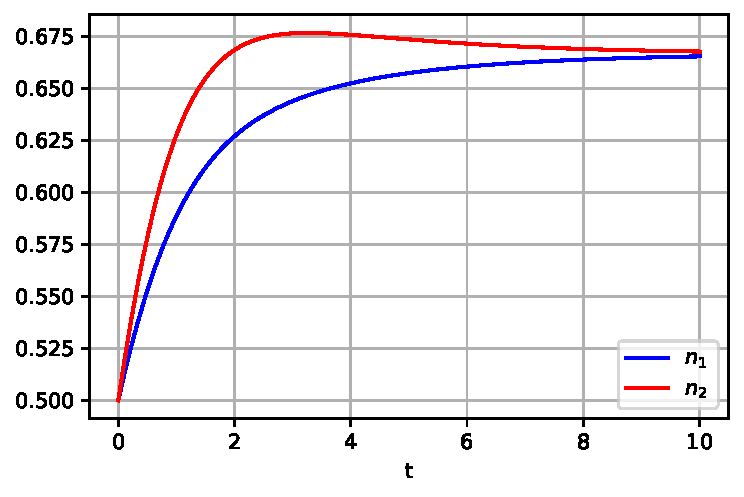
\includegraphics{ContinuousTimeTwoSepcies_files/figure-pdf/fig-compete-numsol-output-1.pdf}

}

\caption{\label{fig-compete-numsol}Numerical solutions of competition
model}

\end{figure}

\begin{figure}

{\centering 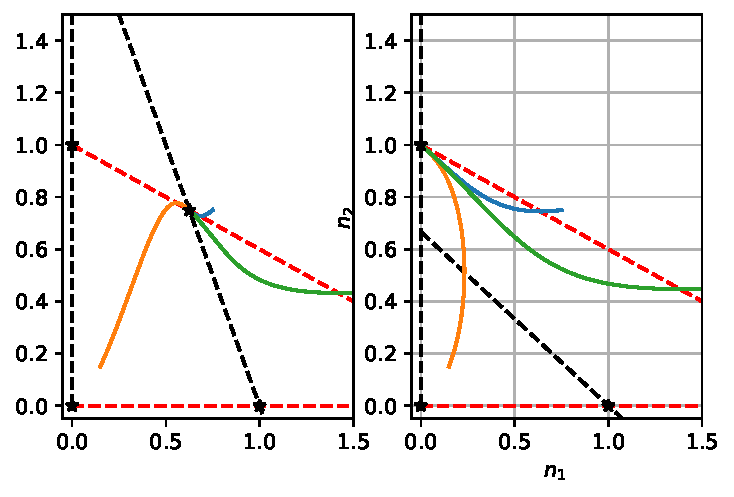
\includegraphics{ContinuousTimeTwoSepcies_files/figure-pdf/fig-comp-numsol-phplane-output-1.pdf}

}

\caption{\label{fig-comp-numsol-phplane}Numerical solution of the
competition model}

\end{figure}

\hypertarget{insight}{%
\subsection{Insight}\label{insight}}

The model therefore has four qualitatively different behaviours that are
described as follows: Consider the case where \(a_{21}>1\). This
represents the case of Population 1 strongly competing with Population
2.

\begin{itemize}
\tightlist
\item
  If \(a_{12}>1\), Population 2 also strongly competes with Population
  1. In this case, there are four biologically relevant steady states,
  two of which are stable (1,0) and (0,1). The coexistence steady state
  is a saddle and thus unstable. The model is bistable and the initial
  conditions determine whether solutions end up at (1,0) or (0,1) (see
  Figure~\ref{fig-comp-numsol-phplane}). The biological interpretation
  of this solution is that one species will always win and completely
  outcompete the other. Even if the two populations are equal
  (\(K_1=K_2\) and \(a_{21}=a_{12}>1\)), one species will always win and
  the other will become extinct.
\item
  If \(a_{12}<1\), Population 2 weakly competes with Population 1. There
  is no coexistence steady state and the only stable steady state is
  (1,0). Hence Population 1 always wins and Population 2 always becomes
  extinct.
\end{itemize}

Now consider the case where \(a_{21}<1\). This represents the case of
Population 1 weakly competing with Population 2.

\begin{itemize}
\tightlist
\item
  If \(a_{12}>1\), Population 2 strongly competes with Population 1.
  There is nonexistence steady state and the only stable steady state is
  (0,1). Hence Population 2 always wins and Population 1 always becomes
  extinct.
\item
  If \(a_{12}<1\), Population 2 also weakly competes with Population 1.
  The coexistence steady state is stable and the steady states (1,0) and
  (0,1) are unstable.
\end{itemize}

\hypertarget{symbiosismutualism}{%
\section{Symbiosis/Mutualism}\label{symbiosismutualism}}

When the interactions between two species results in mutually benefit,
it is known as mutualism or symbiosis. To study this behaviour, we
consider a model of the form \[
\begin{aligned}
\frac{d N_1}{dt} &= r_1N_1\left(1-\frac{N_1}{K_1}+b_{12}\frac{N_2}{K_1}\right), \nonumber \\
\frac{d N_2}{dt} &= r_2N_2\left(1-\frac{N_2}{K_2}+b_{21}\frac{N_1}{K_2}\right). 
\end{aligned}
\] Note the only difference with the competition model is that the sign
of the interaction term has changed. Hence we will not work through all
the details as the analysis is the same as before.

\hypertarget{nondimensionalisation-4}{%
\subsection{Nondimensionalisation}\label{nondimensionalisation-4}}

Using the same nondimensionalisation as the competition model, we obtain
the nondimensional equations
\begin{equation}\protect\hypertarget{eq-mutualismnondim}{}{\begin{aligned}
\frac{d n_1}{d\tau} &= n_1(1- n_1+a_{12}n_2) = f(n_1,n_2), \nonumber \\
\frac{d n_2}{d\tau} &= \rho n_2(1-n_2+a_{21}n_1) =g(n_1,n_2).
\end{aligned}
}\label{eq-mutualismnondim}\end{equation}

\hypertarget{steady-states-3}{%
\subsection{Steady states}\label{steady-states-3}}

This model has steady-states \((0,0)\), \((1,0)\),\((0,1)\) and\\
\[
\left({n_1}^*,{n_2}^*\right)=\left(\frac{1+a_{12}}{1-a_{12}a_{21}},\frac{1+a_{21}}{1-a_{12}a_{21}}\right).
\] The coexistence steady state is biological relevant if
\(a_{12}a_{21}<1\)

\hypertarget{nullclines-2}{%
\subsection{Nullclines}\label{nullclines-2}}

The \(n_1\) nullclines satisfy \[
n_1=0, \ \ \ n_2=\frac{1}{a_{12}}(n_1-1).
\] The \(n_2\) nullclines satisfy \[
n_2=0, \ \ \ n_2=1+a_{21}n_1.
\] Note that both nullclines have a positive slope.

\hypertarget{linear-stability-5}{%
\subsection{Linear stability}\label{linear-stability-5}}

Using a similar analysis to the competition model, it can be shown that
the steady states (0,0), (1,0) and (0,1) are unstable. When
\(a_{12}a_{21}<1\) there is a stable coexistence steady state. See
Figure~\ref{fig-sym-numsol-phplane}.

\begin{verbatim}
/Users/pmurray/anaconda3/lib/python3.11/site-packages/scipy/integrate/_odepack_py.py:248: ODEintWarning:

Excess work done on this call (perhaps wrong Dfun type). Run with full_output = 1 to get quantitative information.
\end{verbatim}

\begin{figure}

{\centering 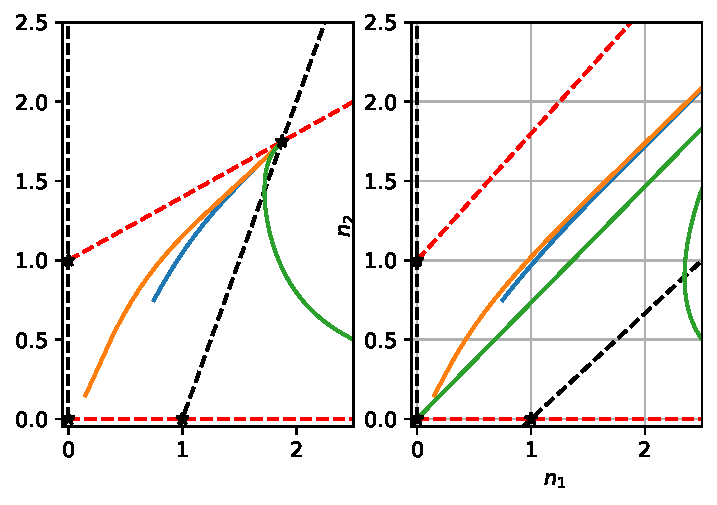
\includegraphics{ContinuousTimeTwoSepcies_files/figure-pdf/fig-sym-numsol-phplane-output-2.pdf}

}

\caption{\label{fig-sym-numsol-phplane}Numerical solution of the
symbiosis model}

\end{figure}

\hypertarget{insight-1}{%
\subsection{Insight}\label{insight-1}}

The important parameter in the model is the product \(a_{12}a_{21}\).
This quantifies the total amount of cooperativity in the model. All
steady states that involve the extinction of a species are unstable. In
the case where if \(a_{12}a_{21}<1\) there is a stable steady state.
Note that steady states of both variables are higher than they would be
in the absence of the other species. In the \(a_{12}a_{21}>1\) there is
no coexistence steady state and both populations grow in an unbounded
manner.

\hypertarget{biochemical-kinetics}{%
\chapter{Biochemical kinetics}\label{biochemical-kinetics}}

Biochemical kinetics concern the concentration of chemical substances in
biological systems. In this section we neglect spatial variation in
concentrations, effectively assuming chemical reactions occur in
environments that are ``well-mixed''.

\hypertarget{the-law-of-mass-action}{%
\section{The law of mass action}\label{the-law-of-mass-action}}

We denote the \(i^{th}\) chemical species using the notation \(C_i\).
The concentration of molecule type \(C_i\) is denoted \([C_i]\) and
represents the number of molecules of \(C_i\) per unit volume.

Suppose \(C_1,..C_M\) undergo the reaction

\[
\lambda_1C_1+\lambda_2 C_2+...+\lambda_m C_M \xrightleftharpoons[k_{b}]{k_{f}} 
 \gamma_1 C_1+\gamma_2 C_2 + ... \gamma_M C_M.
\]

the law of mass action states that the forward reaction proceeds at rate

\[
k_f[C_1]^\lambda_1 [C_2]^\lambda_2 ..[C_M]^\lambda_M
\]

whilst the backward reaction proceeds at rate

\[
k_b[C_1]^\gamma_1[C_2]^\gamma_2 ..[C_M]^\gamma_M
\]

where \(k_f\) and \(k_b\) are dimensional rate constants.

\begin{tcolorbox}[enhanced jigsaw, bottomtitle=1mm, rightrule=.15mm, colback=white, leftrule=.75mm, title=\textcolor{quarto-callout-note-color}{\faInfo}\hspace{0.5em}{Note}, bottomrule=.15mm, coltitle=black, toptitle=1mm, breakable, colframe=quarto-callout-note-color-frame, titlerule=0mm, toprule=.15mm, opacitybacktitle=0.6, arc=.35mm, colbacktitle=quarto-callout-note-color!10!white, left=2mm, opacityback=0]

Suppose A and B react to produce C. Hence \[
A+B\xrightarrow{k}  C.
\]

The law of mass action states that the rate of the reaction is

\[
k[A][B].
\]

Using the reaction rates, we write down ordinary differential equations
that describe how concentrations of a given molecule will change in
time. Hence

\[
\frac{d[C]}{dt}=k[A][B].
\]

\end{tcolorbox}

\begin{tcolorbox}[enhanced jigsaw, bottomtitle=1mm, rightrule=.15mm, colback=white, leftrule=.75mm, title=\textcolor{quarto-callout-note-color}{\faInfo}\hspace{0.5em}{Note}, bottomrule=.15mm, coltitle=black, toptitle=1mm, breakable, colframe=quarto-callout-note-color-frame, titlerule=0mm, toprule=.15mm, opacitybacktitle=0.6, arc=.35mm, colbacktitle=quarto-callout-note-color!10!white, left=2mm, opacityback=0]

Consider the reversible reaction \[
A+B  \xrightleftharpoons[k_{-}]{k_{+}}  C.
\] Define dependent variables, identify reaction rates and derive
ordinary differential equations that describe how concentrations evolved
in time.

The dependent variables are: \[ [A](t), \ \ [B](t), \ \ [C](t) \].

Applying the law of mass action yields the reaction rates:

\[ k_+[A][B] \ \ \textrm{and} \ \ k_-[C]\].

The ODEs are

\[
\begin{aligned}
\frac{d[A]}{dt}&=-k_+[A][B]+k_-[C], \nonumber\\
\frac{d[B]}{dt}&=-k_+[A][B]+k_-[C], \nonumber\\
\frac{d[C]}{dt}&=k_+[A][B]-k_-[C]. \nonumber
\end{aligned}
\]

For a given set of initial conditions, \[
[A](t=0)=[A]_0, \ \ \ [B](t=0)=[B]_0, \ \ \ [C](t=0)=[C]_0,
\] the ODEs can be solved and hence the concentrations of the different
molecules described as time evolves.

\end{tcolorbox}

\hypertarget{example}{%
\subsection{Example}\label{example}}

The previous example have had stochiometric constants all set to unity
(i.e.~all reactions involved a molecules of one species interaction with
one from another). Consider the reaction in which one molecule of
species A with \(m\) of species B giving rise to \(n\) molecules of
species B and \(p\) molecules of species C, i.e. \[
A+mB \xrightarrow{k_1} nB + pC.
%X \underset{k_2}{\stackrel{k_1}{\rightleftharpoons}} Y
\]

The law of mass action says that the rate of the forward reaction is \[
k_1[A][B]^m.
\]

The governing ODEs are \[
\begin{aligned}
\frac{d[A]}{dt}&=-k_1[A][B]^m, \nonumber\\
\frac{d[B]}{dt}&=(n-m)k_1[A][B]^m, \nonumber\\
\frac{d[C]}{dt}&=pk_1[A][B]^m.  \nonumber
\end{aligned}
\]

\begin{tcolorbox}[enhanced jigsaw, bottomtitle=1mm, rightrule=.15mm, colback=white, leftrule=.75mm, title=\textcolor{quarto-callout-note-color}{\faInfo}\hspace{0.5em}{Note}, bottomrule=.15mm, coltitle=black, toptitle=1mm, breakable, colframe=quarto-callout-note-color-frame, titlerule=0mm, toprule=.15mm, opacitybacktitle=0.6, arc=.35mm, colbacktitle=quarto-callout-note-color!10!white, left=2mm, opacityback=0]

Consider the reversible reaction \[
A+A  \xrightleftharpoons[k_{-}]{k_{+}}  B.
\] Define dependent variables, identify reaction rates and derive
ordinary differential equations that describe how concentrations evolved
in time.

The reaction rates are \[
k_+[A]^2
\] and \[
k_- [B].
\] The ODEs are \[
\begin{aligned}
\frac{d[A]}{dt}&=-2k_+[A]^2+2k_- [B] , \nonumber\\
\frac{d[B]}{dt}&=k_+[A]^2-k_- [B], 
\end{aligned}
\]

\end{tcolorbox}

\hypertarget{enzyme-kinetics}{%
\section{Enzyme kinetics}\label{enzyme-kinetics}}

Biochemical reactions are often regulated by enzymes (substances that
convert a substrate into another substrate). Consider a chemical
reaction in which substrate, \(S\), reacts with an enzyme, \(E\), to
form a complex, \(C\). Suppose the complex can either undergo the
reverse reaction or go on to form a product, \(P\), with the release of
the enzyme, i.e. \[
S+E  \xrightleftharpoons[k_{-1}]{k_{1}}  C \xrightarrow{k_2} P+E .
\]

\hypertarget{deriving-the-model-equations}{%
\subsection{Deriving the model
equations}\label{deriving-the-model-equations}}

For notational convenience we let lower case letter denote
concentrations, i.e.~

\[
s(t)=[S](t),  \ \ c(t)=[C](t) , \\ e(t)=[E](t), \\ p(t)=[P](t).
\]

Applying the law of mass action the above enzyme kinetic scheme can be
described by the system of ODES

\begin{equation}\protect\hypertarget{eq-mmenten4var}{}{
\begin{aligned}
\frac{d s}{dt} &= -k_1 se + k_{-1}c, \nonumber \\
\frac{d e}{dt} &= -k_1 se + k_{-1}c +k_2 c,  \nonumber\\
\frac{d c}{dt} &= k_1 se - k_{-1}c-k_2c, \nonumber \\
\frac{d p}{dt} &= k_2 c.
\label{MMenten4Var}
\end{aligned}
}\label{eq-mmenten4var}\end{equation}

We consider initial conditions such that at \(t=0\) the reaction has not
yet started, i.e.~there is no product or complex formed \[
s(0)=s_0, \ \ e(0)=e_0, \ \ c(0)=0, \ \ p(0)=0,
\] where \(s_0\) and \(e_0\) represent the initial concentrations of
substrate and enzyme, respectively.

\hypertarget{reducing-the-dimensions-of-the-model}{%
\subsection{Reducing the dimensions of the
model}\label{reducing-the-dimensions-of-the-model}}

Whilst there are four dependent variables in the problem (\(s(t)\),
\(c(t)\), \(e(t)\) and \(p(t)\)), the description of the problem can be
simplified by noting that the variable \(p(t)\) does not couple back to
the other variables, i.e.~if we can solve the system for \(s(t)\),
\(e(t)\) and \(c(t)\) then \(c(t)\) can be expressed as a function of
time and

\[
p(t)=k_2\int c(t) dt + C_1.
\]

Furthermore, there is a conserved quantity in the system. Note that

\[
\frac{d e}{dt}+\frac{d c}{dt}=0,
\]

which reflects the fact that enzyme exists either in free form or bound
to the product. Integrating yields

\[
c(t)+e(t)=C_2.
\]

Evaluating at \(t=0\),

\[
e_0=C_2.
\]

Hence

\[
c(t)+e(t)=e_0
\]

and the variable \(e(t)\) can be replaced by

\[
 e(t)=e_0-c(t)
\]

Given \[
 e(t)=e_0-c(t),
\] substitute in \[
\begin{aligned}
\frac{d s}{dt} &= -k_1 se + k_{-1}c, \nonumber \\
\frac{d c}{dt} &= k_1 se - k_{-1}c-k_2c, \nonumber \\
\end{aligned}
\] Hence \[
\begin{aligned}
\frac{d s}{dt} &= -k_1 s(e_0-c) + k_{-1}c, \nonumber \\
\frac{d c}{dt} &= k_1 s(e_0-c) - (k_{-1}+k_2)c, \nonumber \\
\end{aligned}
\]

\hypertarget{the-quasi-steady-state-approximation-qssa}{%
\subsection{The quasi-steady state approximation
(QSSA)}\label{the-quasi-steady-state-approximation-qssa}}

A usual approach to these equations is to assume that the timescale of
complex dynamics is very fast compared to that of substrate dynamics.

To make the QSSA we assume that one of the variables (in this case
\(c\)), is in equilibrium

\[
dc/dt \sim 0.
\]

In which case the second equation yields

\[
c=\frac{e_0s(t)}{s(t)+K_m}, 
\]

where

\[
 K_m=\frac{k_{-1}+k_2}{k_1},
\]

is known as the Michaelis constant.

Now consider \[
\begin{aligned}
\frac{d s}{dt} &= -k_1 s(e_0-c) + k_{-1}c, \nonumber \\
\end{aligned}
\] By QSSA \[
-k_1 s(e_0-c) + k_{-1}c=-k_2c=-k_2\frac{e_0s(t)}{s(t)+K_m},
\] Hence \[
\begin{aligned}
\frac{d s}{dt} &= -k_2\frac{e_0s(t)}{s(t)+K_m}, \nonumber \\
\end{aligned}
\] Note this could be achieved by direct substitution for \(c(t)\).

\hypertarget{enzyme-kinetics-the-michaelis-menten-quasi-steady-state-approximation-qssa}{%
\subsection{Enzyme kinetics: the Michaelis-Menten quasi-steady state
approximation
(QSSA)}\label{enzyme-kinetics-the-michaelis-menten-quasi-steady-state-approximation-qssa}}

\hypertarget{nondimensionalisation-5}{%
\subsubsection{Nondimensionalisation}\label{nondimensionalisation-5}}

Nondimensionalisation using \[
\tau=k_1 e_0 t, \ \ \ u=\frac{s}{s_0}, \ \ \ v=\frac{c}{e_0},
\] yields the ODEs
\begin{equation}\protect\hypertarget{eq-mmenten2varnondim}{}{
\begin{aligned}
\frac{d u}{d\tau} &= -u+(u+K-\lambda)v, \nonumber \\
\epsilon \frac{d v}{d\tau} &= u-(u+K)v, \nonumber \\
\end{aligned}
}\label{eq-mmenten2varnondim}\end{equation}

where \[
\lambda=\frac{k_2}{k_1 s_0}, \ \ \ K=\frac{k_{-1}+k_2}{k_1 s_0}, \ \ \ \epsilon=\frac{e_0}{s_0}. 
\]

\hypertarget{asymptotic-expansions-the-outer-solution}{%
\subsubsection{Asymptotic expansions: the outer
solution}\label{asymptotic-expansions-the-outer-solution}}

We consider the (often realised) case where the amount of enzyme in the
system is small compared with the amount of substrate, i.e. \[
\epsilon \ll 1.
\] The presence of the small parameter \(\epsilon\) allows us to use
perturbation theory to calculate approximate solutions to
Equation~\ref{eq-mmenten2varnondim}. However, the problem is singular
owing to the \(\epsilon dv/dt\) term.

We propose an outer solution of the form

\[
\begin{aligned}
u(\tau;\epsilon)=u_0(\tau) + \epsilon u_1(\tau) + \epsilon^2 u_2(\tau) + ... = \sum_{n=0}^{\infty}u_n(\tau)\epsilon^n, \nonumber \\
v(\tau;\epsilon)=v_0(\tau) + \epsilon v_1(\tau) + \epsilon^2 v_2(\tau) + ... = \sum_{n=0}^{\infty}v_n(\tau)\epsilon^n.  \nonumber  
\end{aligned}
\]

Substituting the expansions in Equation~\ref{eq-mmenten2varnondim}
yields

\[
\begin{aligned}
\frac{du_0}{d\tau} + \epsilon \frac{du_1}{d\tau} + \epsilon^2\frac{du_2}{d\tau} + ... = -(u_0(\tau) + \epsilon u_1(\tau) + \epsilon^2 u_2(\tau) + ...)+  \nonumber \\ (u_0(\tau) + \epsilon u_1(\tau) + \epsilon^2 u_2(\tau) + ...+ K-\lambda)(v_0(\tau) + \epsilon v_1(\tau) + \epsilon^2 v_2(\tau) + ...).  \nonumber 
\end{aligned}
\]

Gathering terms as coefficients of the different powers of \(\epsilon\)
yields

\[
\begin{aligned}
\frac{du_0}{d\tau} + \epsilon \frac{du_1}{d\tau} + ... = -u_0(\tau)+ (u_0(\tau)+ K-\lambda)v_0  +\epsilon (-u_1(\tau) + u_1v_0+v_1u_0+v_1(K-\lambda)) + O(\epsilon^2), \nonumber
\end{aligned}
\]

where terms of order \(\epsilon^2\) have been neglected.

Considering the \(v\) equation yields

\[
\begin{aligned}
\epsilon(\frac{dv_0}{d\tau} + \epsilon \frac{dv_1}{d\tau} + \epsilon^2\frac{dv_2}{d\tau} + ..) = u_0(\tau) + \epsilon u_1(\tau) + \epsilon^2 u_2(\tau) + ...  \nonumber \\ -(u_0(\tau) + \epsilon u_1(\tau) + \epsilon^2 u_2(\tau) + ...+ K) (v_0(\tau) + \epsilon v_1(\tau) + \epsilon^2 v_2(\tau) + ...).  \nonumber 
\end{aligned}
\]

Gathering terms as coefficients of the different powers of \(\epsilon\)
yields

\[
\begin{aligned}
\epsilon\frac{dv_0}{d\tau} + \epsilon^2 \frac{dv_1}{d\tau} + ... = u_0(\tau)-   u_0(\tau)v_0(\tau) -v_0 K  \nonumber \\ +\epsilon (u_1(\tau) - u_0v_1 - u_1v_0 - Kv_1) + O(\epsilon^2).  \nonumber 
\end{aligned}
\]

At \(O(1)\)

\[
\begin{aligned}
\frac{du_0}{d\tau} = -u_0+ (u_0+ K-\lambda)v_0  \nonumber \\ 
 0= u_0 - u_0 v_0 -v_0K.    \nonumber
\end{aligned}
\]

Solving the algebraic equation yields

\[
v_0=\frac{u_0}{u_0+K},
\]

and substituting in the \(u_0\) equation yields

\[
\frac{du_0}{d\tau} = -u_0+ (u_0+ K-\lambda)\frac{u_0}{u_0+K} = -\frac{\lambda u_0}{u_0+K}.
\]

Integrating yields

\[
u_0+K\ln u_0=-\lambda \tau +A,
\]

where \(A\) is an integration constant.

When posing a solution as an expansion, a necessary question to ask is
when the expansion is a valid? On the outer scale we have shown that \[
v_0=\frac{u_0}{u_0+K}.
\]

Note that the expression

\[
v_0=\frac{u_0}{u_0+K}
\]

does not satisfy the initial condition \(v(0)=0\). As \(u_0(0)=1\), we
find that at \(\tau=0\)

\[
v_0=\frac{1}{1+K} \neq 0.
\]

Hence the proposed expansion is not valid at least near \(\tau=0\).

\hypertarget{asymptotic-expansions-the-inner-solution}{%
\subsubsection{Asymptotic expansions: the inner
solution}\label{asymptotic-expansions-the-inner-solution}}

This issue can be rectified by proposing a different scaling for time
and recalculating a series solution in the new coordinate system.

We proceed by making the change of variable \[
\sigma=\frac{\tau}{\epsilon}.
\]

Note that \(\sigma=1\) corresponds to \(\tau=\epsilon\). Hence the
proposed rescaling of time will give rise to what is called the inner
solution to the problem (close to \(t=0\)).

To distinguish inner and outer solutions we relabel dependent variables
such that

\[
\begin{aligned}
u(\tau;\epsilon)=U(\sigma;\epsilon),  \nonumber \\ 
v(\tau;\epsilon)=V(\sigma;\epsilon). \nonumber 
\end{aligned}
\]

Note that \[
\frac{d}{d\tau}=\frac{1}{\epsilon}\frac{d}{d\sigma}.
\] Hence upon changing variables \[
\begin{aligned}
\frac{1}{\epsilon}\frac{d U}{d\sigma} &= -\epsilon U+ \epsilon (U+K-\lambda)V, \nonumber \\
\frac{1}{\epsilon}\ \epsilon \frac{d V}{d\sigma} &= U-(U+K)V.  
\end{aligned}
\]

Upon tidying \begin{equation}\protect\hypertarget{eq-longtimeuv}{}{
\begin{aligned}
\frac{d U}{d\sigma} &= -\epsilon U+ \epsilon (U+K-\lambda)V, \nonumber \\
\frac{d V}{d\sigma} &= U-(U+K)V.  
\end{aligned}
}\label{eq-longtimeuv}\end{equation}

We seek series solutions to Equation~\ref{eq-longtimeuv} of the form

\[
\begin{aligned}
U(\sigma;\epsilon)&=U_0(\sigma) + \epsilon U_1(\sigma) + \epsilon^2 U_2(\sigma) + ... = \sum_{n=0}^{\infty}U_n(\sigma)\epsilon^n, \nonumber \\
V(\sigma;\epsilon)&=V_0(\sigma) + \epsilon V_1(\sigma) + \epsilon^2 V_2(\sigma) + ... = \sum_{n=0}^{\infty}V_n(\sigma)\epsilon^n. \nonumber  
\end{aligned}
\]

Substitution yields \[
\begin{aligned}
\frac{dU_0}{d\sigma}+ \epsilon\frac{dU_1}{d\sigma}+ ..... &= \epsilon\left( U_0+\epsilon U_1 + ... + (U_0+\epsilon U_1+ +K-\lambda)(V_0+\epsilon V_1+...)\right) \\
\frac{dV_0}{d\sigma}+ \epsilon\frac{dV_1}{d\sigma}+ ..... &= (U_0+\epsilon U_1+...)-(U_0+\epsilon U_1+...+K)(V_0+\epsilon V_1+...).
\end{aligned}
\]

Hence at leading order \[
\begin{aligned}
\frac{dU_0}{d\sigma}&=0  \nonumber\\
\frac{dV_0}{d\sigma}&=U_0-(U_0+K)V_0.
\end{aligned}
\]

Given the initial condition \(U(0)=1\) we obtain that the inner solution
is

\[
U(\sigma)=1.
\]

Substituting in the second equation gives

\[
 \frac{dV_0}{d\sigma}=1-(1+K)V_0.
\]

Given \(V_0(0)=0\) we obtain

\[
V_0=\frac{1-e^{-(1+K)\sigma}}{1+K}.
\]

\hypertarget{asymptotic-expansions-matching-the-inner-and-outer-solutions}{%
\subsubsection{Asymptotic expansions: matching the inner and outer
solutions}\label{asymptotic-expansions-matching-the-inner-and-outer-solutions}}

Inner and outer solutions are matched by taking limits \[
\lim_{\tau \rightarrow 0}(u_0(\tau),v_0(\tau))=\lim_{\sigma \rightarrow \infty}(U_0(\sigma),V_0(\sigma)).
\]

Note that

\[
\lim_{\sigma\rightarrow \infty} V_0(\sigma)= \lim_{\sigma\rightarrow \infty}  \frac{1-e^{-(1+K)\sigma}}{1+K} = \frac{1}{1+K},
\]

and

\[
\lim_{\tau\rightarrow 0}(v_0(\tau)) =\lim_{\tau\rightarrow 0}\frac{u_0}{u_0+K} =  \frac{1}{1+K}. 
\]

Hence the \(v\) variables are already matching in the appropriate limit.

Similarly

\[
\lim_{\sigma\rightarrow \infty} U_0(\sigma)= 1,
\]

hence we require that

\[
\lim_{\tau \rightarrow 0} u_0(\tau)= 1.
\]

Hence for

\[
 (u_0+K\ln u_0=-\lambda \tau +A)
\]

to hold as \(\tau \rightarrow 0\) implies \(A=1\).

\hypertarget{the-brusselator}{%
\section{The Brusselator}\label{the-brusselator}}

The Brusselator is an abstract model that can be used to demonstrate
oscillations in (bio)-chemical systems. Consider a chemical reaction
where five chemical species, A, B, D, X and Y, react according to the
scheme \[
\begin{aligned}
A&\xrightarrow{k_{1}} X,  \nonumber \\
B+X&\xrightarrow{k_{2}} Y+D, \nonumber\\
2X+Y&\xrightarrow{k_{3}} 3X, \nonumber\\
X&\xrightarrow{k_{4}} E. 
\end{aligned}
\]

Assuming that the concentration of A and B (\([A]\) and \([B]\),
respectively) are in vast excess (i.e.~the amount that A and B get
depleted by the reactions is negligible compared with the total amount
of A and B present), their concentration are treated as constants.
Furthermore, as D and E are products but not reactants (they only appear
on the right-hand side of reactions) we do not concern ourselves with
their dynamics.

\hypertarget{deriving-model-equations}{%
\subsection{Deriving model equations}\label{deriving-model-equations}}

To make the steps leading to ODEs obvious, it is useful to rewrite the
reaction scheme in the form \[
 \begin{aligned}
A&\xrightarrow{k_{1}} X,  \nonumber \\
B+X&\xrightarrow{k_{2}} Y+D, \nonumber\\
X+X+Y&\xrightarrow{k_{3}} X+X+X, \nonumber\\
X&\xrightarrow{k_{4}} E. 
\end{aligned}
\]

Applying the law of mass action yields that the four reactions occur at
rates:

\begin{itemize}
\tightlist
\item
  \(k_1[A]\),
\item
  \(k_2[B][X]\),
\item
  \(k_3[X]^2[Y]\),
\item
  \(k_4[X]\).
\end{itemize}

The total time derivative of \([X]\) is obtained by visiting each X in
the reaction scheme once and adding the corresponding reaction rate to
the right-hand side of the ODE, i.e.

\[  
 \begin{aligned}
 \frac{d[X]}{dt} &= \overbrace{k_1[A]}^{R1-lhs} - \overbrace{k_2[B][X]}^{R2-lhs} -  \overbrace{k_3[X]^2[Y]}^{R3-lhs} - \overbrace{k_3[X]^2[Y]}^{R3-lhs} + \overbrace{k_3[X]^2[Y]}^{R3-rhs}+ \overbrace{k_3[X]^2[Y]}^{R3-rhs}+ \overbrace{k_3[X]^2[Y]}^{R3-rhs} -\overbrace{k_4[X]}^{R4-lhs}, \nonumber \\
        &= k_1[A] - k_2[B][X] + k_3[X]^2[Y]   -k_4[X]. 
 \end{aligned}
 \]

Similarly for species Y we obtain that the total rate of change in time
is \[ 
 \begin{aligned}
  \frac{d[Y]}{dt}=k_2[B][X]-k_3[X]^2[Y].
 \end{aligned}
\]

\hypertarget{nondimensionalisation-6}{%
\subsection{Nondimensionalisation}\label{nondimensionalisation-6}}

Upon making the change of variables \[
\begin{aligned}
x=\sqrt{\frac{k_3}{k_4}}[X], \ \ \ \ \ y=\sqrt{\frac{k_3}{k_4}}[Y], \ \ \textrm{and} \ \ \tau=k_4 t, 
\end{aligned}
\] yields \begin{equation}\protect\hypertarget{eq-brussnondim}{}{
\begin{aligned}
\frac{d x}{d \tau} &= a-bx+x^2y-x = f(x,y), \\
\frac{d y}{d \tau} &= bx-x^2y = g(x,y), 
\end{align}
}\label{eq-brussnondim}\end{equation}

where \[
a=[A]\frac{k_1}{k_4}\sqrt{\frac{k_3}{k_4}} \ \ \ \textrm{and} \ \ \ b= [B]\frac{k_2}{k_4}.
\]

\hypertarget{steady-states-analysis}{%
\subsection{Steady states analysis}\label{steady-states-analysis}}

Seeking steady states \((x^*,y^*)\) of equations
Equation~\ref{eq-brussnondim} such that \[
f(x^*,y^*)=g(x^*,y^*)=0
\] yields

\[
(x^*,y^*)=(a,\frac{b}{a}).
\]

\hypertarget{linear-stability-analysis-5}{%
\subsection{Linear stability
analysis}\label{linear-stability-analysis-5}}

The Jacobian matrix is

\[
A=\left(\begin{array}{rr}
\frac{\partial f}{\partial x}&\frac{\partial f}{\partial y} \\ \frac{\partial g}{\partial x }&\frac{\partial g}{\partial y} \end{array}\right) = \left(\begin{array}{rr}
-b+2xy-1&x^2\\ b-2xy &-x^2\end{array}\right).
\]

Evaluating the Jacobian at \((a,b/a)\) yields

\[
A=
 \left(\begin{array}{rr}
b-1&a^2\\ -b &-a^2\end{array}\right). 
\]

The determinant of the Jacobian is

\[
\det{A}=-(b-1)a^2+a^2b=a^2>0,
\]

Hence \((a,b/a)\) is not a saddle. The trace of the Jacobian is \[
\mathrm{tr} A=b-1-a^2.
\]

Hence if \(b>1+a^2\) the trace is positive and, referring to
Figure~\ref{fig-tdplane}, the steady state is linearly unstable.
Otherwise, the steady state is linearly stable.

In Figure~\ref{fig-bruss-numsol} we numerically solve
Equation~\ref{eq-brussnondim} in the case of oscillatory solutions. Note
that when the steady state is unstable, the numerical solution indicates
that the system has limit cycle solutions. A valid question to ask is
whether one can prove that this is the case.

\begin{figure}

{\centering 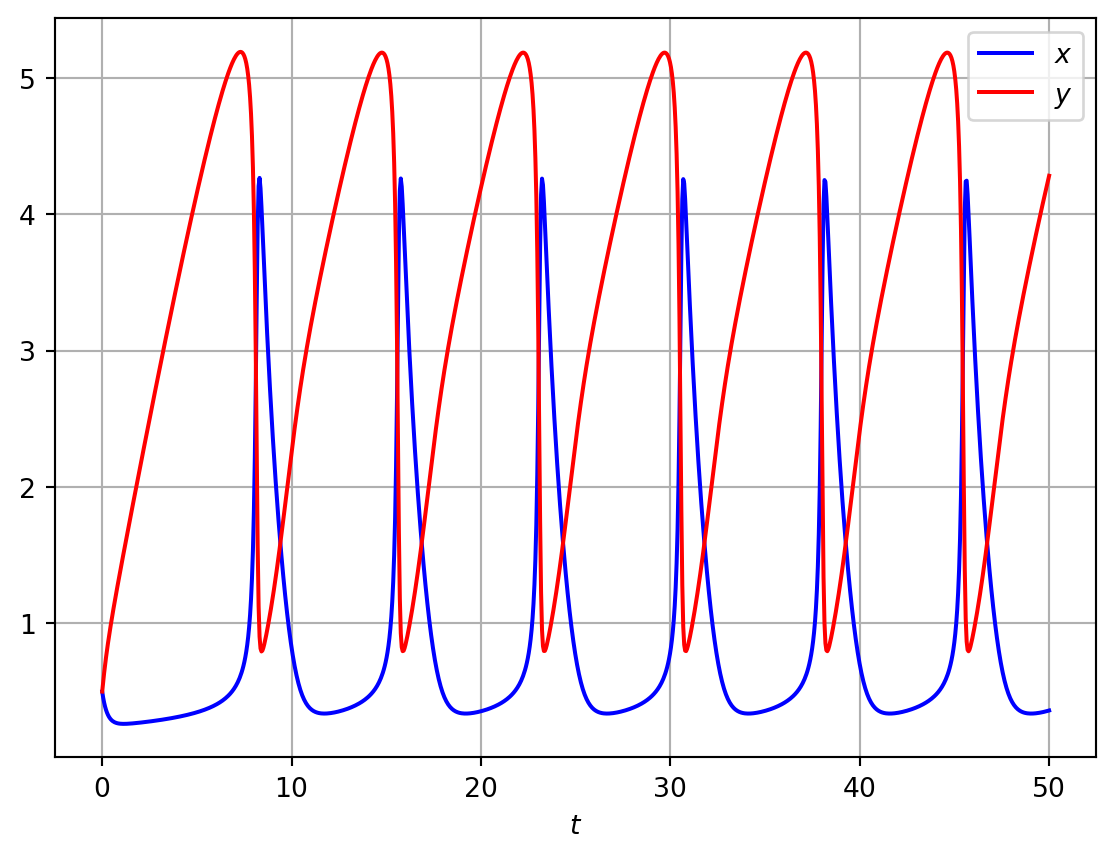
\includegraphics{enzymekinetics_files/figure-pdf/fig-bruss-numsol-output-1.pdf}

}

\caption{\label{fig-bruss-numsol}Numerical solutions of the Brusselator
model}

\end{figure}

\begin{figure}
\centering
\subfigure[]{\includegraphics[scale=0.3]{BrusselatorOsc.eps}}
\subfigure[]{\includegraphics[scale=0.3]{BrusselatorStable.eps}}
\caption{Solutions of the Brusselator equations in the oscillatory (a) and stable (b) regimes. Parameter values are: (a) $a=1.5$, $b=1.15(a^2+1)$, (a) $a=1.5$, $b=0.95(a^2+1)$. Initial conditions: $x(0)=1.05$, $y(0)=1.05$.}
\label{BrussNondimFig}
\end{figure}

\hypertarget{applying-the-poincaire-bendixson-theorem}{%
\subsection{Applying the Poincaire-Bendixson
theorem}\label{applying-the-poincaire-bendixson-theorem}}

Recall that the Poincaire-Bendixson theorem can be used to prove the
existence of limit cycle solutions in a case where a bounding set
encloses a single unstable steady state. Hence given the case of the
Brusselator with \(b>a^2+1\), the identification of a bounding set will
allow application of the Poincaire-Bendixson theorem and hence prove the
existence of limit cycle solutions.

We begin by defining the nullclines of the system. The \(x\) nullcline
is given by

\[
y=\frac{1+b}{x}-\frac{a}{x^2}.
\]

The \(y\) nullclines are given by

\[
y=\frac{b}{x} \ \ \ \textrm{and} \ \ \ x=0.
\]

In the positive quadrant, this nullcline has a single root at
\(a/(1+b)\), tends to 0 as \(x\rightarrow \infty\) and has a maximum at
\(x=2a/(1+b)\).

\begin{figure}

{\centering 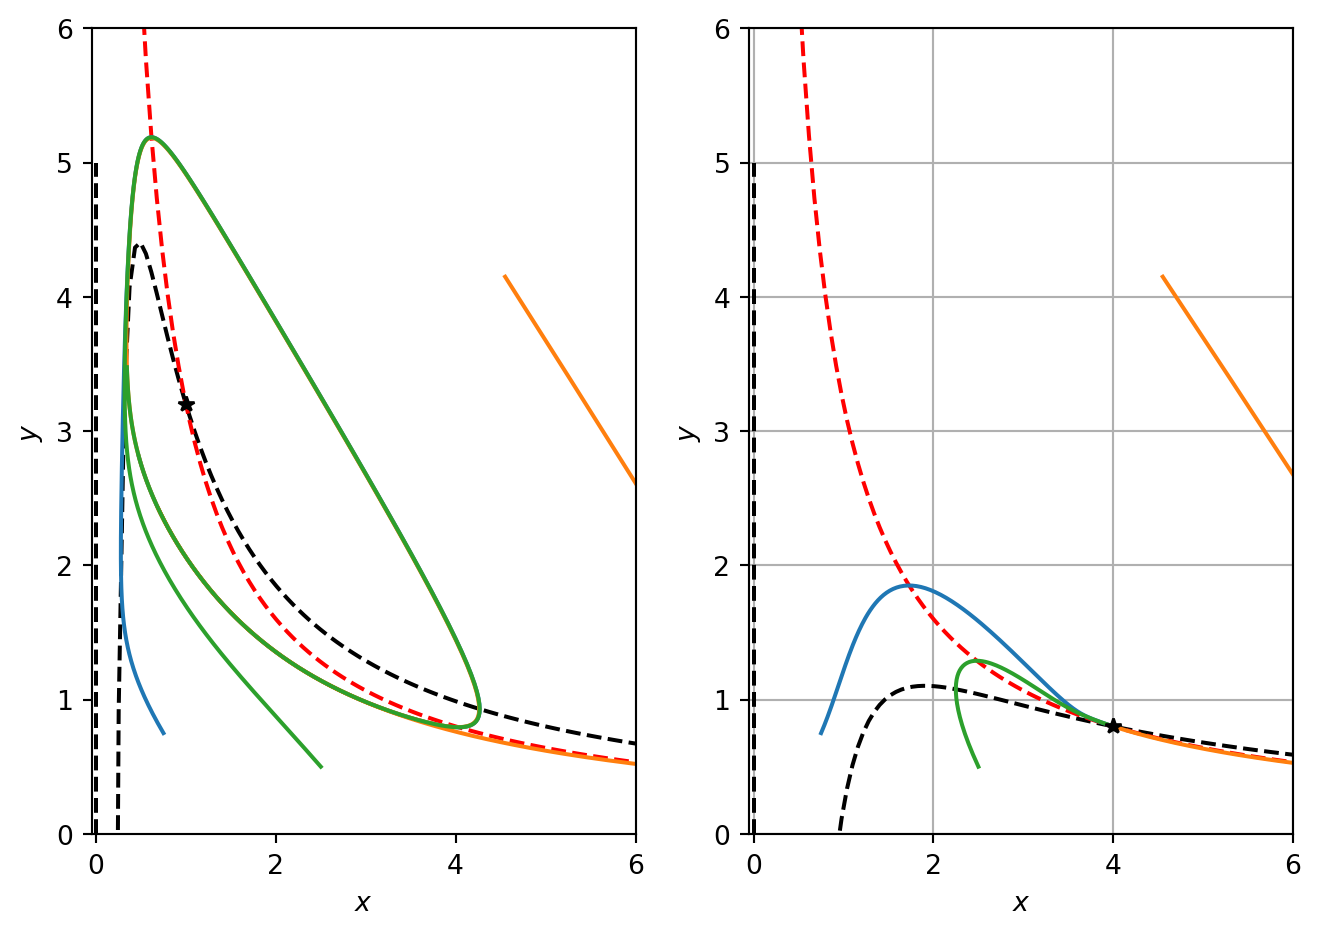
\includegraphics{enzymekinetics_files/figure-pdf/fig-bruss-numsol-phplane-output-1.pdf}

}

\caption{\label{fig-bruss-numsol-phplane}Numerical solution of the
Brusselator.}

\end{figure}

In Figure~\ref{fig-bruss-numsol-phplane} we plot the the oscillatory
solution together with the nullclines. Note that the nullclines separate
the phase plane into regions of constant sign. Note that the \(x\)
nullcline separates the phase plane into regions where \(dx/dt>0\) and
\(dx/dt<0\). Similarly, the \(y\) nullcline separates the phase plane
into regions where \(dy/dt>0\) and \(dy/dt<0\).

Note that signs for \(dx/dt\) can be determined by considering behaviour
of the function \(f\) as one moves away from the nullcline where, by
definition, \(f=0\). Consider some point that sits on the x nullcline.
While keeping the \(x\) value fixed, increase \(y\) so the point moves
vertically in the phase plane. This implies that \(f\) has increased
because the only term to change is \(x^2y\). Hence \(f\) increases upon
increasing \(y\) and therefore \(dx/dt\) is positive for all points
above the \(x\) nullcline. Alternatively, note that in the Jacobian
matrix we have calculated that \(\partial f/\partial y\) is positive.

\hypertarget{a-confined-set}{%
\subsubsection{A confined set}\label{a-confined-set}}

To define a confined set, we construct the closed loop ABCDEA in phase
space (see Figure~\ref{fig-bruss-numsol-phplane-confinedset}) where the
points A, B, C, D and E are defined as follows. Let the points A and B
be two points on the \(x\) axis with coordinates \((\delta,0)\) and
\((a/(1+b),0)\), respectively. We choose \(\delta>a\). The outward
normal to the line segment AB is \(\mathbf{n}=[0,-1]\). To show that the
trajectories point inwards along AB, we compute

\[
\mathbf{n}.[\frac{dx}{dt},\frac{dy}{dt}] = -\frac{dy}{dt}.
\]

As the line segment AB sits below the \(y\) nullcline, \(dy/dt>0\) in
this region. Hence

\[
\mathbf{n}.[\frac{dx}{dt},\frac{dy}{dt}] = -\frac{dy}{dt}<0.
\]

Hence trajectories point inwards on the line segment AB.

Let \(C\) represent the point \[
(a/(1+b),b(1+b)/a).
\]

The normal vector to the line segment BC is \(\mathbf{n}=[-1,0]\). As BC
lies to the left of the \(x\) nullcline, in a region where \(dx/dt>0\),
then

\[
\mathbf{n}.[\frac{dx}{dt},\frac{dy}{dt}] = -\frac{dx}{dt}<0.
\]

Hence trajectories point inwards on the line segment BC.

Consider the line segment CD where D has coordinates \[
(k,b(1+b)/a),
\] with \(k>a\)

The normal to this line segment is {[}0,1{]}. As CD lies in a region of
the phase plane where \(dy/dt<0\),

\[
\mathbf{n}.[\frac{dx}{dt},\frac{dy}{dt}] = \frac{dy}{dt}<0.
\] Hence trajectories point inwards on the line segment CD.

Let E be a point that sits on the \(x\) nullcline at some position \[
(\delta,(\delta(1+b)-a)/(\delta^2)),
\] such that DE is a straight line with outwardly pointing normal vector
\([1,1]\). Along DE

\[
\mathbf{n}.[\frac{dx}{dt},\frac{dy}{dt}] =   a-bx+x^2y-x + bx-x^2y = a-x<0
\]

for \(x>a\). As \(k>a\), \(x>a\) for all points on DE, hence
trajectories point inwards on DE.

Finally, consider the line segment EA which has normal vector
\(\mathbf{n}=[1,0]\). As \(dx/dt<0\) along EA

\[
\mathbf{n}.[\frac{dx}{dt},\frac{dy}{dt}] =  \frac{dx}{dt} <0.
\]

\begin{figure}

{\centering 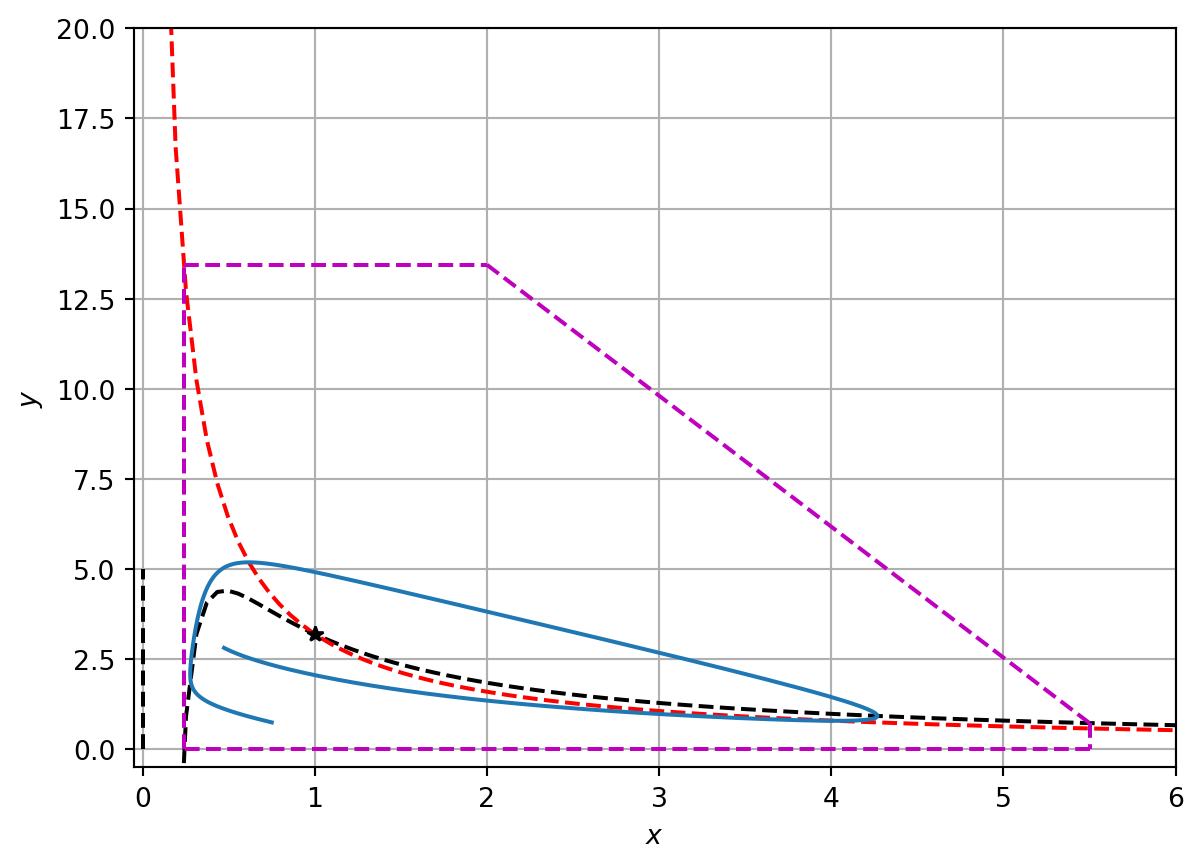
\includegraphics{enzymekinetics_files/figure-pdf/fig-bruss-numsol-phplane-confinedset-output-1.pdf}

}

\caption{\label{fig-bruss-numsol-phplane-confinedset}Numerical solution
of the Brusselator.}

\end{figure}

Hence at all points on the closed loop ABCDEA trajectories point inwards
(see Figure~\ref{fig-bruss-numsol-phplane-confinedset}). Hence ABDCEA is
a confined set and the Poincaire-Bendixson theorem states that the
system exhibits limit cycle solutions when the steady state is unstable.
This is precisely the behaviour that we see numerically in Figure
Figure~\ref{fig-bruss-numsol-phplane}.

\hypertarget{refs}{}
\begin{CSLReferences}{1}{0}
\leavevmode\vadjust pre{\hypertarget{ref-britton2003essential}{}}%
Britton, Nicholas F, and NF Britton. 2003. \emph{Essential Mathematical
Biology}. Vol. 453. Springer.

\leavevmode\vadjust pre{\hypertarget{ref-edelstein2005mathematical}{}}%
Edelstein-Keshet, Leah. 2005. \emph{Mathematical Models in Biology}.
SIAM.

\leavevmode\vadjust pre{\hypertarget{ref-ludwig1978qualitative}{}}%
Ludwig, Donald, Dixon D Jones, Crawford S Holling, et al. 1978.
{``Qualitative Analysis of Insect Outbreak Systems: The Spruce Budworm
and Forest.''} \emph{Journal of Animal Ecology} 47 (1): 315--32.

\leavevmode\vadjust pre{\hypertarget{ref-murray2002mathematical}{}}%
Murray, J. D. 2002. \emph{Mathematical Biology i: An Introduction}.
Springer.

\end{CSLReferences}



\end{document}
